\section{Casi d'uso}
Vengono elencati i casi d'uso rilavati dall'analisi del capitolato C5 e durante le riunioni con Zucchetti S.P.A.. \\
Ogni caso d'uso è identificato da seguente formalismo:
\begin{center}
	UC[codice]
\end{center}
dove il codice indica il codice univoco di ogni caso d'uso che verrà riportato in forma gerarchica.

\subsection{Attori}
Di seguito è riportato il diagramma \textit{UML\ped{G}} che descrive la gerarchia degli attori. Dopo un'attenta analisi da parte del \textit{team\ped{G}} sono state individuate 3 tipologie differenti di attori con funzionalità crescenti. Gli attori sono: l'utente non autenticato, l'utente autenticato e infine l'utente autenticato pro.
\label{Attori}
\begin{figure}
	\centering
	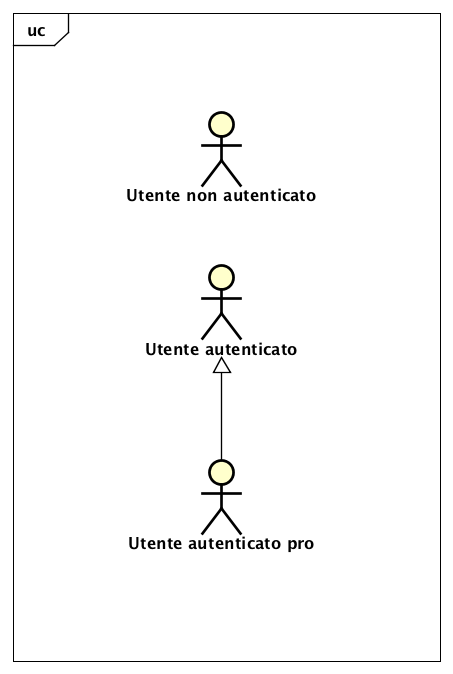
\includegraphics[scale=0.45]{UML/attori.png}
	\caption{Attori dell'applicazione}
\end{figure}


\subsection{Caso d'uso UC1: Scenario principale}
\begin{center}
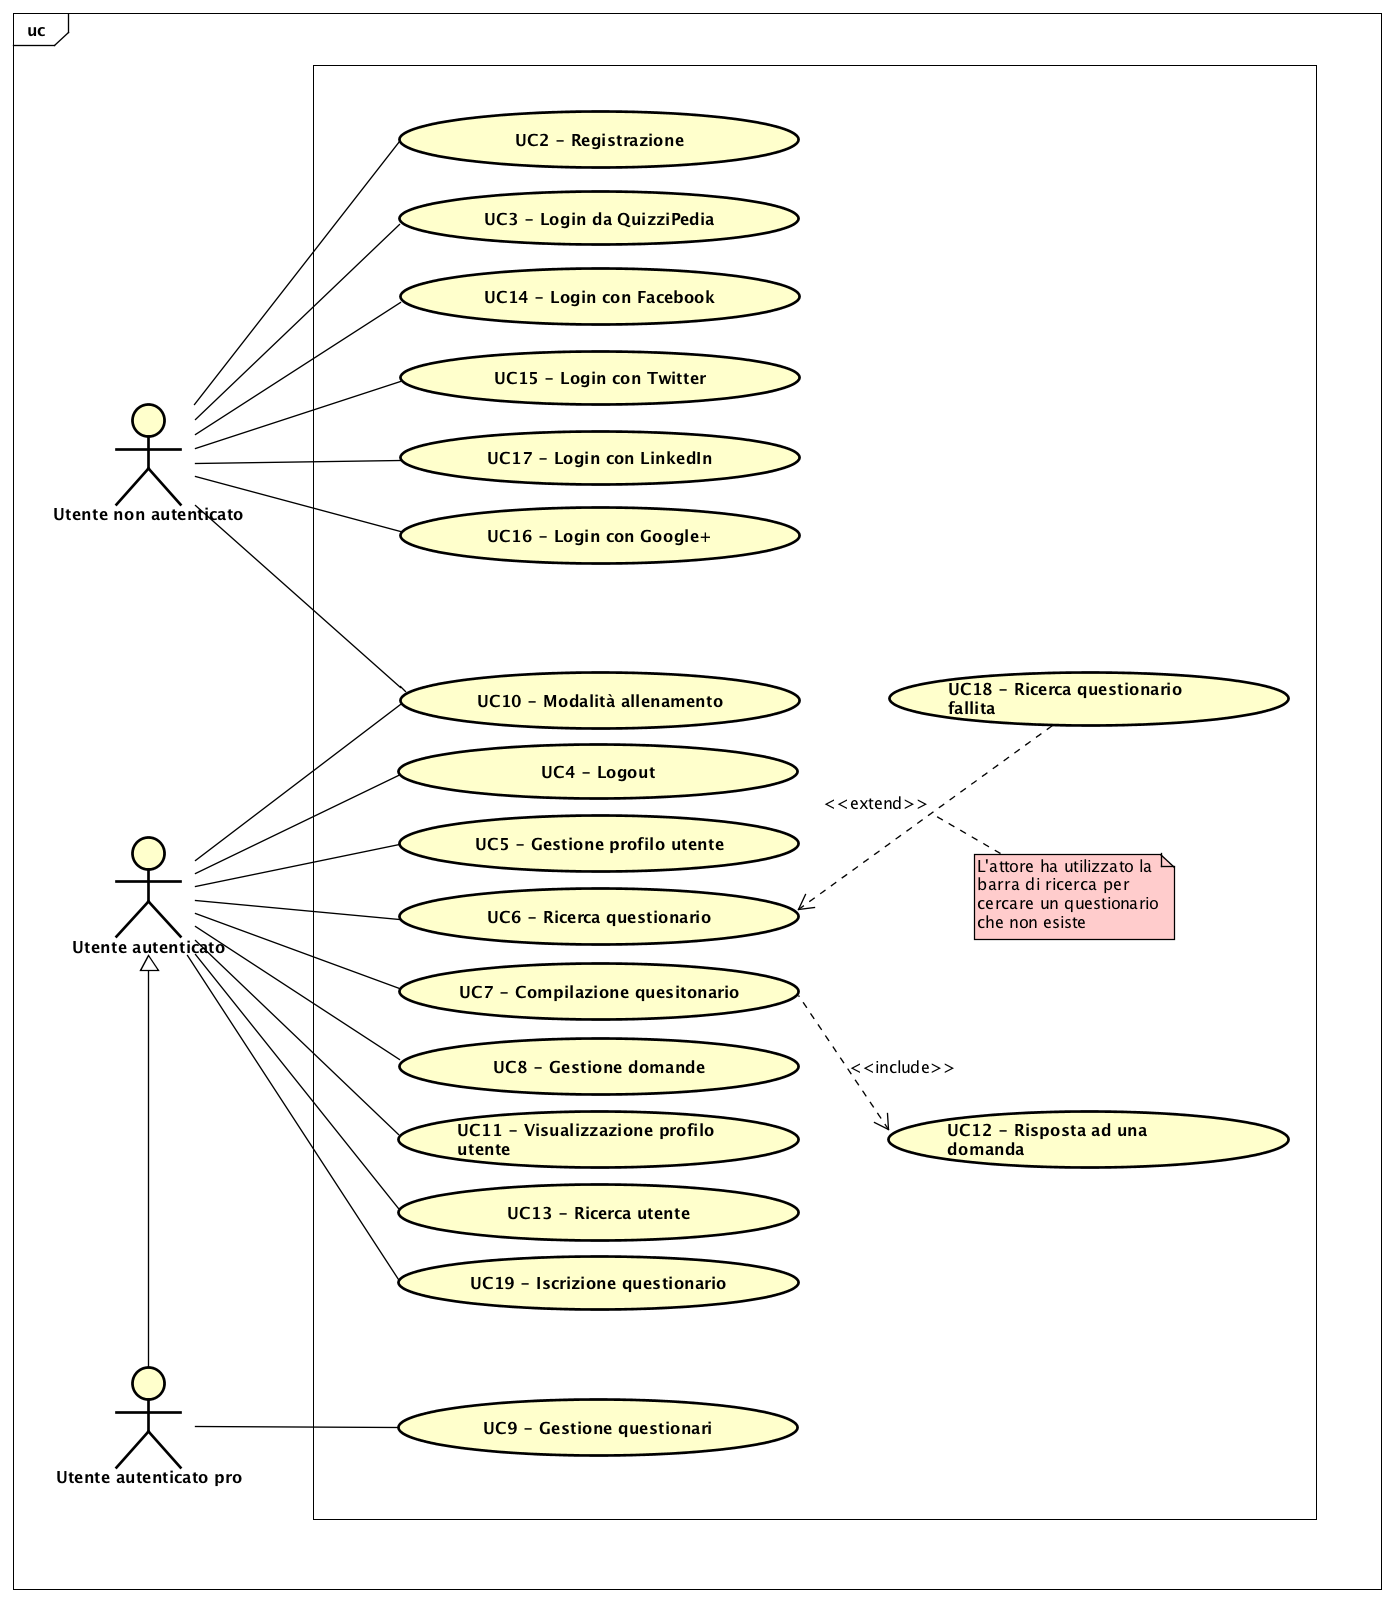
\includegraphics[scale=0.5]{UML/UC1.png}
\end{center}
\begin{itemize}
\item\textbf{Attori}: utente, utente autenticato, utente autenticato pro;
\item\textbf{Descrizione}: nella schermata principale un utente non autenticato può ricercare e compilare questionari pubblici esistenti. Può inoltre autenticarsi tramite l'apposito form di login oppure registrarsi.\\
L'utente autenticato, oltre a svolgere tutte le operazioni dell'utente non autenticato, è abilitato a:
\begin{itemize}
\item Effettuare il logout;
\item Gestire il proprio profilo: modificare il proprio nome, cognome, indirizzo e-mail e password. Può visualizzare i questionari realizzati, compilati e consultare le relative valutazioni ricevute;
\item Gestire le domande: inserire nuove domande nel sistema oppure eliminarne una da lui creata;
\item Gestire i questionari: creare questionari pubblici oppure eliminare un questionario da lui creato.
\end{itemize}

L'utente autenticato pro può, oltre a svolgere tutte le operazioni dell'utente autenticato, gestire questionari privati. E abilitato dunque a creare, modificare e proporre questionari privati destinati ad un numero limitato di utenti;
\item\textbf{Pre-condizione}: il sistema è avviato e mostra la pagina iniziale dell'applicazione;
\item\textbf{Post-condizione}: il sistema ha ricevuto tutte le informazioni dall'utente sulle operazioni che vuole eseguire.
\item\textbf{Scenario principale}:
\begin{itemize}
\item L'utente può registrarsi all'applicazione (UC2);
\item L'utente può eseguire il login all'applicazione (UC3);
\item L'utente autenticato/autenticato pro può eseguire il logout dall'applicazione (UC4); 
\item L'utente autenticato/autenticato pro può gestire il proprio profilo utente (UC5);
\item L'utente autenticato/autenticato pro può ricercare questionari esistenti (UC6);
\item L'utente autenticato/autenticato pro può compilare un questionario  selezionato (UC7);
\item L'utente autenticato/autenticato pro può gestire le domande (UC8);
\item L'utente autenticato/autenticato pro può gestire i questionari (UC9).
\end{itemize}
\end{itemize}

\newpage
\subsection{Caso d'uso UC2: Registrazione}
\begin{center}
	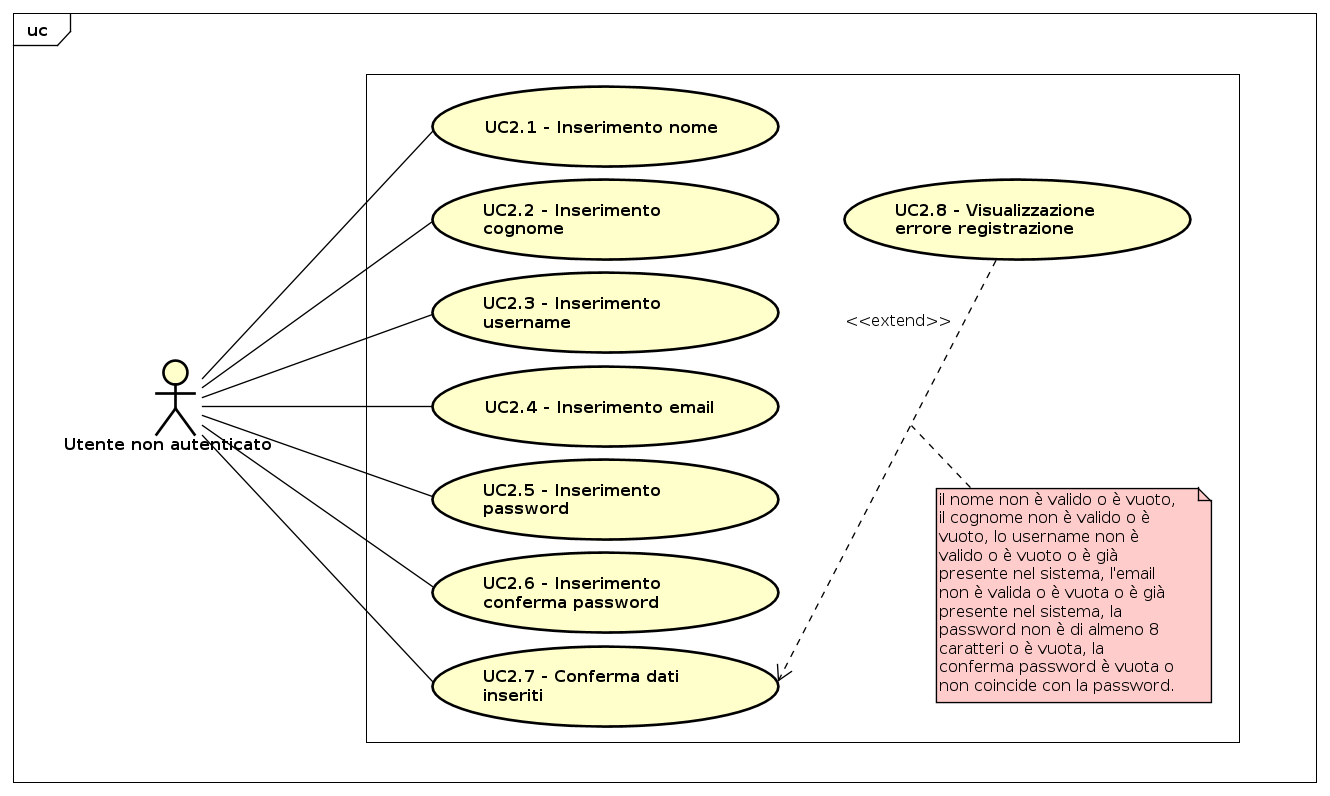
\includegraphics[scale=0.5]{UML/UC2.png}
\end{center}
\begin{itemize}
\item \textbf{Attori}: Utente;
\item \textbf{Scopo e descrizione}: per poter usufruire dei servizi forniti dalla piattaforma, l'utente deve registrarsi inserendo email e password;
\item \textbf{Precondizione}: il sistema è avviato e mostra la pagina iniziale;
\item \textbf{Scenario principale}:
	\begin{enumerate}
	\item L'utente inserisce il proprio nome (UCD2.1);
	\item L'utente inserisce il proprio cognome (UCD2.2);
	\item L'utente sceglie uno username (UCD2.3);
	\item L'utente inserisce l'email (UCD2.4);
	\item L'utente inserisce la password (UCD2.5);
	\item L'utente inserisce una seconda volta la password (UCD2.6);
	\item L'utente conferma i dati inseriti (UCD2.7).
	\end{enumerate}
\item \textbf{Scenario alternativo}: possono verificarsi uno o più dei seguenti scenari:
	\begin{itemize}
	\item[-] Il nome inserito non è valido oppure è vuoto;
	\item[-] Il cognome inserito non è valido oppure è vuoto;
	\item[-] Lo username inserito non è valido oppure è vuoto;
	\item[-] Lo username inserito è già presente nel sistema;
	\item[-] L'email inserita non è valida oppure è vuota;
	\item[-] L'email inserita è già presente nel sistema;
	\item[-] La password inserita è vuota oppure non è di almeno 8 caratteri;
	\item[-] La password e la conferma password non coincidono.
	\end{itemize}
In tal caso il sistema ritorna allo stato precedente l'inserimento dei dati visualizzando un messaggio di errore;
\item \textbf{Estensione}: l'utente visualizza un messaggio di errore (UCD2.8).
\item \textbf{Postcondizione}: il sistema ha registrato l'utente.
\end{itemize}

\subsubsection{Caso d'uso UC2.1: Inserimento nome}
\begin{itemize}
\item \textbf{Attori}: Utente;
\item \textbf{Scopo e descrizione}: l'utente inserisce il proprio nome per potersi registrare;
\item \textbf{Precondizione}: il sistema presenta all'utente lo spazio destinato a questa operazione;
\item \textbf{Postcondizione}: il nome è stato inserito.
\end{itemize}

\subsubsection{Caso d'uso UC2.2: Inserimento cognome}
\begin{itemize}
\item \textbf{Attori}: Utente;
\item \textbf{Scopo e descrizione}: l'utente inserisce il proprio cognome per potersi registrare;
\item \textbf{Precondizione}: il sistema presenta all'utente lo spazio destinato a questa operazione;
\item \textbf{Postcondizione}: il cognome è stato inserito.
\end{itemize}

\subsubsection{Caso d'uso UC2.3: Inserimento username}
\begin{itemize}
\item \textbf{Attori}: Utente;
\item \textbf{Scopo e descrizione}: l'utente inserisce il proprio username per potersi registrare;
\item \textbf{Precondizione}: il sistema presenta all'utente lo spazio destinato a questa operazione;
\item \textbf{Postcondizione}: lo username è stato inserito.
\end{itemize}

\subsubsection{Caso d'uso UC2.4: Inserimento email}
\begin{itemize}
\item \textbf{Attori}: Utente;
\item \textbf{Scopo e descrizione}: l'utente inserisce il proprio indirizzo email per potersi registrare;
\item \textbf{Precondizione}: il sistema presenta all'utente lo spazio destinato a questa operazione;
\item \textbf{Postcondizione}: l'email è stata inserita.
\end{itemize}

\subsubsection{Caso d'uso UC2.5: Inserimento password}
\begin{itemize}
\item \textbf{Attori}: Utente;
\item \textbf{Scopo e descrizione}: l'utente inserisce una password a sua scelta per potersi registrare;
\item \textbf{Precondizione}: il sistema presenta all'utente lo spazio destinato a questa operazione;
\item \textbf{Postcondizione}: la password è stata inserita.
\end{itemize}

\subsubsection{Caso d'uso UC2.6: Inserimento conferma password}
\begin{itemize}
\item \textbf{Attori}: Utente;
\item \textbf{Scopo e descrizione}: l'utente inserisce nuovamente la password scelta;
\item \textbf{Precondizione}: il sistema presenta all'utente lo spazio destinato a questa operazione;
\item \textbf{Postcondizione}: la conferma della password è stata inserita.
\end{itemize}

\subsubsection{Caso d'uso UC2.7: Conferma registrazione}
\begin{itemize}
\item \textbf{Attori}: Utente;
\item \textbf{Scopo e descrizione}: l'utente conferma i dati inseriti;
\item \textbf{Precondizione}: il sistema presenta all'utente lo spazio destinato a questa operazione;
\item \textbf{Postcondizione}: il sistema ha ricevuto i dati per la registrazione.
\end{itemize}

\subsubsection{Caso d'uso UC2.8: Visualizzazione errore registrazione}
\begin{itemize}
\item \textbf{Attori}: Utente;
\item \textbf{Scopo e descrizione}: l'utente visualizza un messaggio d'errore nel caso si fossero verificati uno o più scenari alternativi;
\item \textbf{Precondizione}: il sistema ha ricevuto dei dati errati per la registrazione;
\item \textbf{Postcondizione}: il sistema mostra un messaggio di errore.
\end{itemize}


\newpage
\subsection{Caso d'uso UC3: Login}
\label{UC3}
\begin{figure}
	\centering
	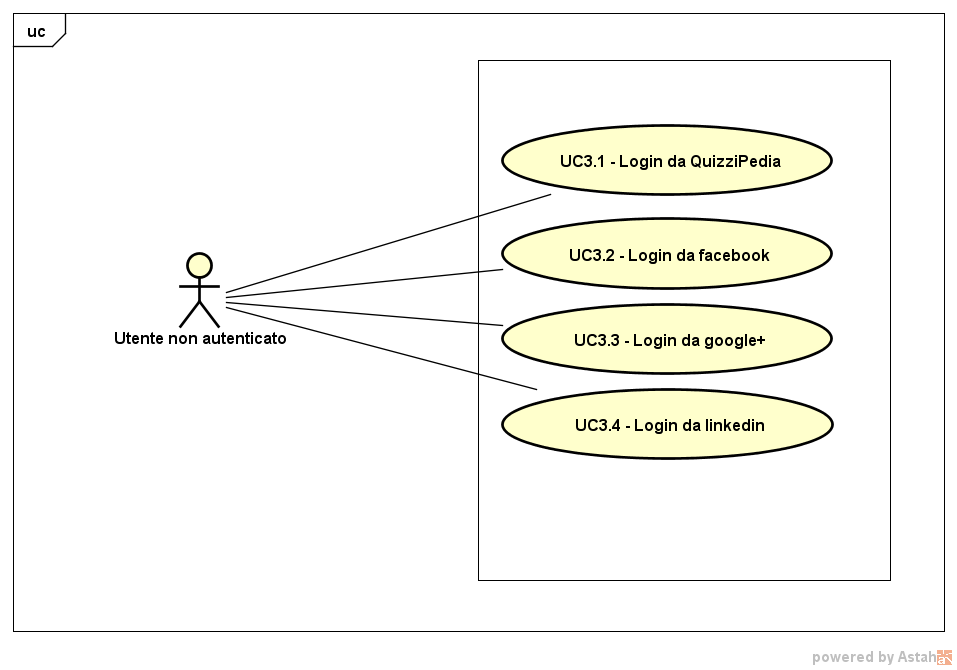
\includegraphics[scale=0.5]{UML/UC3.png}
	\caption{UC3: Login}
\end{figure}
\FloatBarrier
\begin{itemize}
	\item \textbf{Attori}: utente non autenticato;
	\item \textbf{Descrizione}: l'attore si può autenticare tramite uno dei metodi proposti;
	\item \textbf{Precondizione}: il sistema è avviato e pronto per l'utilizzo e mostra la pagina di login;
	\item \textbf{Postcondizione}: l'attore è autenticato;
	\item \textbf{Scenario principale}: l'attore sceglie uno dei seguenti modi per autenticarsi:
		\begin{enumerate}
			\item L'attore può effettuare il login con \progetto (UC3.1);
			\item L'attore può effettuare il login con Facebook (UC3.2);
			\item L'attore può effettuare il login con Twitter (UC3.3);
			\item L'attore può effettuare il login con Google+ (UC3.4);
			\item L'attore può effettuare il login con LinkedIn (UC3.5).
		\end{enumerate}
\end{itemize}

\subsubsection{Caso d'uso UC3.1: Login da \progetto}
\label{UC3.1}
\begin{figure}
	\centering
	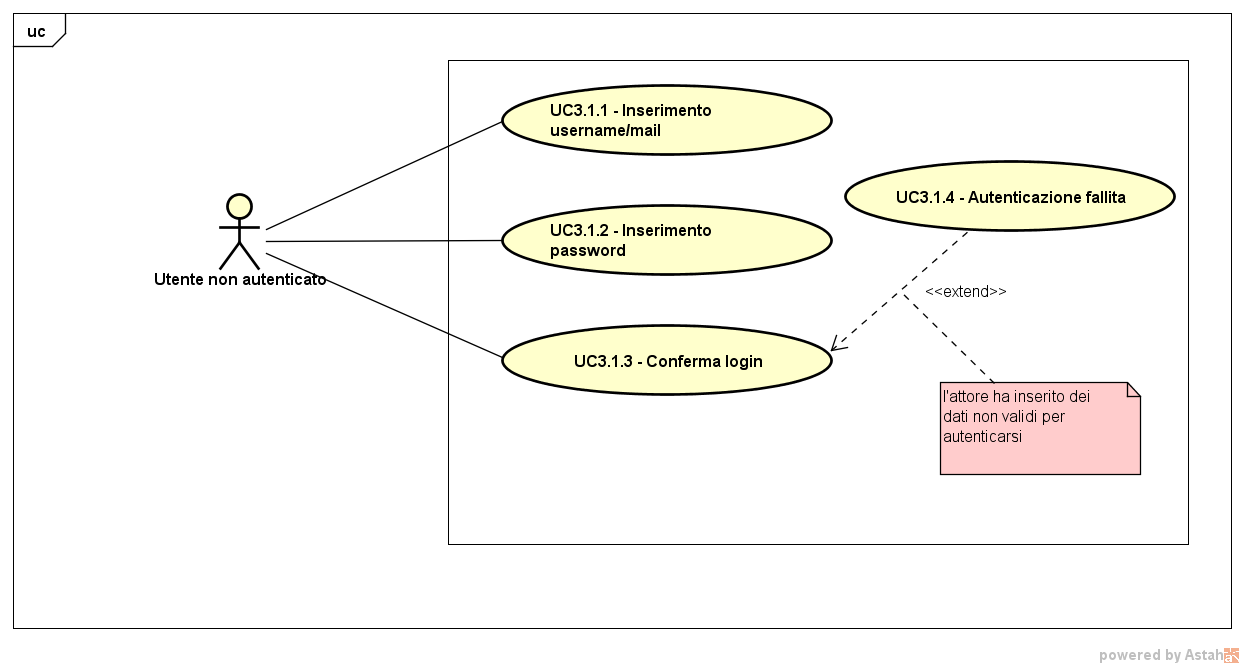
\includegraphics[scale=0.48]{UML/UC3_1.png}
	\caption{UC3.1: Login da \progetto}
\end{figure}
\FloatBarrier
\begin{itemize}
	\item \textbf{Attori}: utente non autenticato;
	\item \textbf{Descrizione}: l'attore si può autenticare inserendo username/mail e password, con cui è registrato;
	\item \textbf{Precondizione}: il sistema è avviato e pronto per l'utilizzo e mostra la pagina di login;
	\item \textbf{Postcondizione}: il sistema ha autenticato l'attore e quindi mostra all'attore autenticato la sua area riservata;
	\item \textbf{Scenario Principale}:
	\begin{enumerate}
		\item L'attore può inserire l'username oppure la mail utilizzata al momento della registrazione (UC3.1.1);
		\item L'attore può inserire la password (UC3.1.2);
		\item L'attore può confermare il login (UC3.1.3).
	\end{enumerate}
	\item \textbf{Estensioni}: autenticazione fallita (UC3.1.4).
\end{itemize}

\subsubsection{Caso d'uso UC3.1.1: Inserimento username/mail}
\begin{itemize}
	\item \textbf{Attori}: utente non autenticato;
	\item \textbf{Descrizione}: l'attore può inserire l'username o la mail associata al proprio account;
	\item \textbf{Precondizione}: il sistema presenta all'attore lo spazio destinato a questa operazione;
	\item \textbf{Postcondizione}: l'attore ha inserito username/mail;
	\item \textbf{Scenario principale}: l'attore inserisce l'username o la mail associata al proprio account. 
\end{itemize}

\subsubsection{Caso d'uso UC3.1.2: Inserimento password}
\begin{itemize}
	\item \textbf{Attori}: utente non autenticato;
	\item \textbf{Descrizione}: l'attore può inserire la password associata al proprio account;
	\item \textbf{Precondizione}: il sistema presenta all'attore lo spazio destinato a questa operazione;
	\item \textbf{Postcondizione}: l'attore inserisce la password;
	\item \textbf{Scenario principale}: l'attore inserisce la password associata al proprio account.
\end{itemize}

\subsubsection{Caso d'uso UC3.1.3: Conferma login}
\begin{itemize}
	\item \textbf{Attori}: utente non autenticato;
	\item \textbf{Descrizione}: l'attore può confermare i dati inseriti per effettuare il login;
	\item \textbf{Precondizione}: l'attore ha inserito l'username/mail e la password;
	\item \textbf{Postcondizione}: l'attore è autenticato;
	\item \textbf{Scenario principale}: l'attore conferma i dati inseriti per effettuare il login con il proprio account.
\end{itemize}

\subsubsection{Caso d'uso UC3.1.4: Autenticazione fallita}
\begin{itemize}
	\item \textbf{Attori}: utente non autenticato;
	\item \textbf{Descrizione}: l'attore può visualizzare un messaggio d'errore nel caso si fossero verificati uno o più scenari alternativi durante la fase di autenticazione;
	\item \textbf{Precondizione}: il sistema ha ricevuto dei dati errati per l'autenticazione;
	\item \textbf{Postcondizione}: il sistema avvisa l'attore dell'errore verificatosi tramite un opportuno messaggio;
	\item \textbf{Scenario principale}: l'attore visualizza un messaggio d'errore.
\end{itemize}

\subsubsection{Caso d'uso UC3.2: Login con Facebook}
\begin{itemize}
	\item \textbf{Attori}: utente non autenticato;
	\item \textbf{Descrizione}: l'attore può autenticarsi utilizzando Facebook;
	\item \textbf{Precondizione}: l'attore visualizza la pagina di login e sceglie il login con Facebook;
	\item \textbf{Postcondizione}: l'attore è autenticato;
	\item \textbf{Scenario principale}: l'attore effettua il login tramite Facebook.
\end{itemize}
\subsubsection{Caso d'uso UC3.3: Login con Twitter}
\begin{itemize}
	\item \textbf{Attori}: utente non autenticato;
	\item \textbf{Scopo e descrizione}: l'attore può autenticarsi utilizzando Twitter;
	\item \textbf{Precondizione}: l'attore visualizza la pagina di login e sceglie il login con Twitter;
	\item \textbf{Postcondizione}: l'attore è autenticato;
	\item \textbf{Scenario principale}: l'attore effettua il login tramite Twitter.
\end{itemize}
\subsubsection{Caso d'uso UC3.4: Login con Google+}
\begin{itemize}
	\item \textbf{Attori}: utente non autenticato;
	\item \textbf{Descrizione}: l'attore può autenticarsi utilizzando Google+;
	\item \textbf{Precondizione}: l'attore visualizza la pagina di login e sceglie il login con Google+;
	\item \textbf{Postcondizione}: l'attore è autenticato;
	\item \textbf{Scenario principale}: l'attore effettua il login tramite Google+.
\end{itemize}
\subsubsection{Caso d'uso UC3.5: Login con LinkedIn}
\begin{itemize}
	\item \textbf{Attori}: utente non autenticato;
	\item \textbf{Descrizione}: l'attore può autenticarsi utilizzando LinkedIn;
	\item \textbf{Precondizione}: l'attore visualizza la pagina di login e sceglie il login con LinkedIn;
	\item \textbf{Postcondizione}: l'attore è autenticato;
	\item \textbf{Scenario principale}: l'attore effettua il login tramite LinkedIn.
\end{itemize}

\subsection{Caso d'uso UC4: Logout}
	\label{UC4}
	\begin{figure}[h]
		\centering
			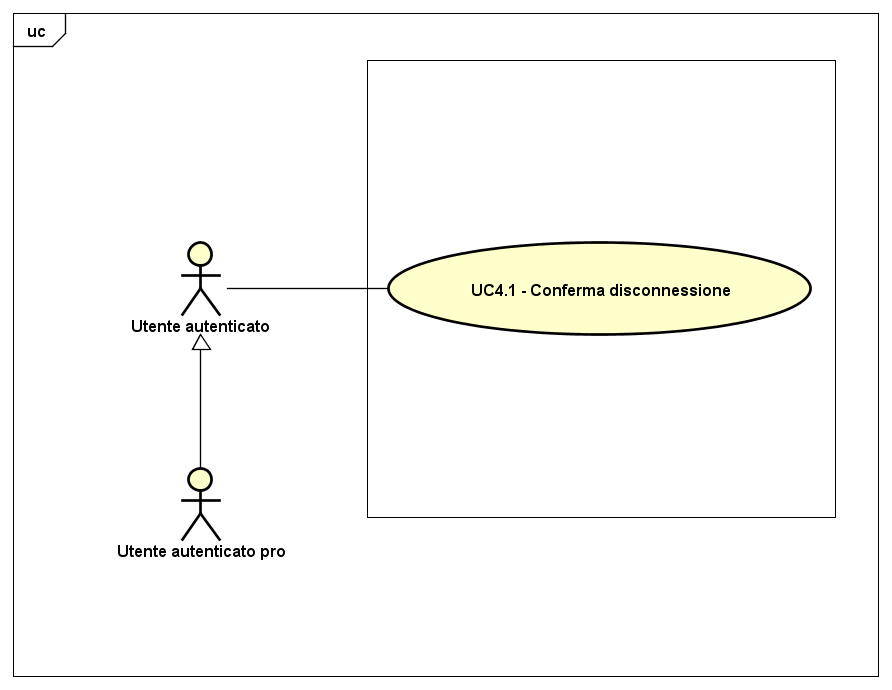
\includegraphics[scale=0.45,keepaspectratio]{UML/UC4.png}
		\caption{UC4: Logout}
	\end{figure}
	\FloatBarrier
	\begin{itemize}
		\item
			\textbf{Attori}: Utente autenticato, utente autenticato pro;
		\item		
			\textbf{Scopo e descrizione}: L'utente autenticato termina la sua sessione, uscendo dalla sua area riservata;
		\item
			\textbf{Pre-condizione}: L'utente è autenticato presso il sistema.
		\item
			\textbf{Post-condizione}: L'utente non è autenticato presso il sistema. 
		\item
			\textbf{Scenario principale}:
	       		\begin{enumerate}
					\item 	
					L'Utente seleziona l'opzione logout per scollegarsi dal sistema [UC4.1];
					\item
					L'Utente riceve la conferma della disconnessione [UC4.2].
	 			\end{enumerate}
	\end{itemize}

\subsubsection{Caso d'uso UC4.1: Selezione opzione logout}
	\begin{itemize}
		\item		
			\textbf{Attori}: Utente Autenticato, utente autenticato pro;
		\item
  			\textbf{Scopo e descrizione}: L'utente seleziona l'opzione logout per poter uscire dalla sua area riservata;
		\item
			\textbf{Pre-condizione}: L'utente è autenticato presso il sistema. 
		\item
			\textbf{Post-condizione}: L'utente non è autenticato presso il sistema.
	\end{itemize}
\subsubsection{Caso d'uso UC4.2: Conferma disconnessione}
	\begin{itemize}
		\item
			\textbf{Attori}: Utente Autenticato, utente autenticato pro;
		\item
			\textbf{Scopo e descrizione}: L'utente una volta selezionato l'opzione logout, attende la conferma della disconnessione da parte del sistema;
 		\item
			\textbf{Pre-condizione}: L'utente autenticato ha selezionato l'opzione logout;
		\item
			\textbf{Post-condizione}: Il sistema conferma all'utente l'uscita dalla sua area riservata.
	\end{itemize}		
	

\newpage
\subsection{Caso d'uso UC5: Gestione profilo utente}

\label{UC5}
\begin{figure}[ht]
	\centering
	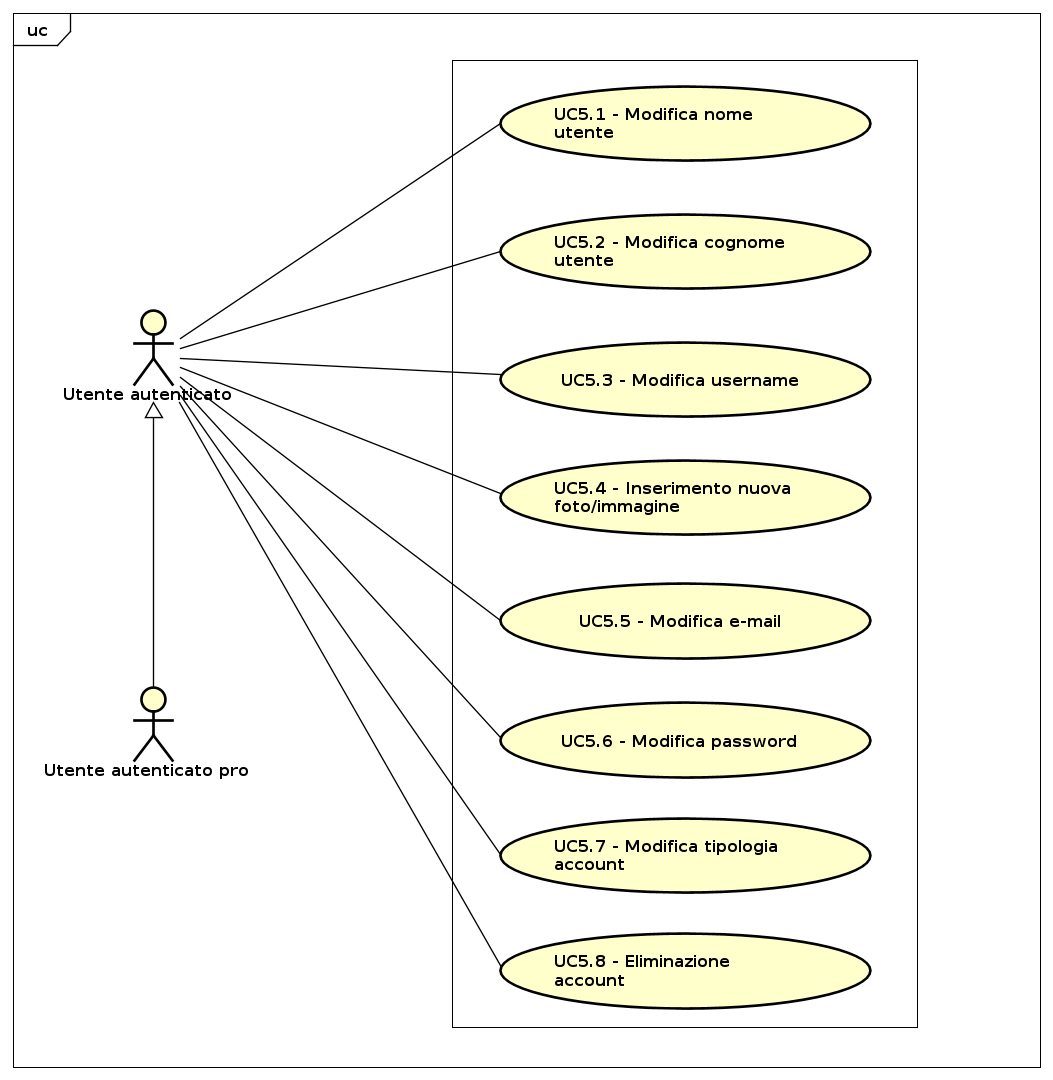
\includegraphics[scale=0.5,keepaspectratio]{UML/UC5.png}
	\caption{UC5: Gestione profilo utente}
\end{figure}
\FloatBarrier
\begin{itemize}
	\item \textbf{Attori}: utente autenticato, utente autenticato pro;
	\item \textbf{Descrizione}: l'attore può visualizzare e modificare i suoi dati personali;
	\item \textbf{Precondizione}: il sistema visualizza l'opzione di gestione profilo utente;
	\item \textbf{Postcondizione}: il sistema ha attuato le modifiche effettuate dall'attore ai propri dati personali;
	\item \textbf{Scenario principale}:
		\begin{enumerate}
			\item L'attore può modificare il proprio nome utente (UC5.1);
			\item L'attore può modificare il proprio cognome utente (UC5.2);
			\item L'attore può inserire una nuova foto/immagine per il proprio profilo utente (UC5.3);
			\item L'attore può modificare la propria e-mail (UC5.4);
			\item L'attore può modificare la propria password (UC5.5);
			\item L'attore può confermare le modifiche effettuate al proprio profilo utente (UC5.6)
			\item L'attore può modificare la tipologia del proprio account (UC5.8);
			\item L'attore può eliminare il proprio account (UC5.9).
		\end{enumerate} 
	\item \textbf{Estensioni}: l'attore visualizza un messaggio d'errore relativo alla conferma della modifica del profilo utente	(UC5.7);	 
\end{itemize}

\subsubsection{Caso d'uso UC5.1: Modifica nome utente}
\begin{itemize}
	\item \textbf{Attori}: utente autenticato, utente autenticato pro;
	\item \textbf{Descrizione}: l'attore può inserire un nuovo nome utente;
	\item \textbf{Precondizione}: il sistema visualizza l'opzione per l'inserimento nome utente;
	\item \textbf{Postcondizione}: l'attore ha inserito il nuovo nome utente;
	\item \textbf{Scenario principale}: l'attore inserisce il nuovo nome utente.
\end{itemize}

\subsubsection{Caso d'uso UC5.2: Modifica cognome utente}
\begin{itemize}
	\item \textbf{Attori}: utente autenticato, utente autenticato pro;
	\item \textbf{Descrizione}: l'attore può inserire un nuovo cognome utente;
	\item \textbf{Precondizione}: il sistema visualizza l'opzione per l'inserimento cognome utente; 
	\item \textbf{Postcondizione}:  l'attore ha inserito il nuovo cognome utente;
	\item \textbf{Scenario principale}: l'attore inserisce il nuovo cognome utente.
\end{itemize}

\subsubsection{Caso d'uso UC5.3: Inserimento foto/immagine}
\begin{itemize}
	\item \textbf{Attori}: utente autenticato, utente autenticato pro;
	\item \textbf{Descrizione}: l'attore può caricare una nuova foto/immagine;
	\item \textbf{Precondizione}: il sistema visualizza l'opzione per caricare una foto/immagine;  
	\item \textbf{Postcondizione}: l'attore ha caricato una nuova foto/immagine;
	\item \textbf{Scenario principale}: l'attore carica una nuova foto/immagine.
\end{itemize}

\subsubsection{Caso d'uso UC5.4: Modifica e-mail}
\begin{itemize}
	\item \textbf{Attori}: utente autenticato, utente autenticato pro;
	\item \textbf{Descrizione}: l'attore può inserire un nuovo indirizzo di posta elettronica;
	\item \textbf{Precondizione}: il sistema visualizza l'opzione per l'inserimento e-mail;
	\item \textbf{Postcondizione}: l'attore ha inserito un nuovo indirizzo di posta elettronica;
	\item \textbf{Scenario principale}: l'attore inserisce un nuovo indirizzo di posta elettronica.
\end{itemize}

\subsubsection{Caso d'uso UC5.5: Modifica password}
\label{UC5.5}
\begin{figure}[h]
	\centering
	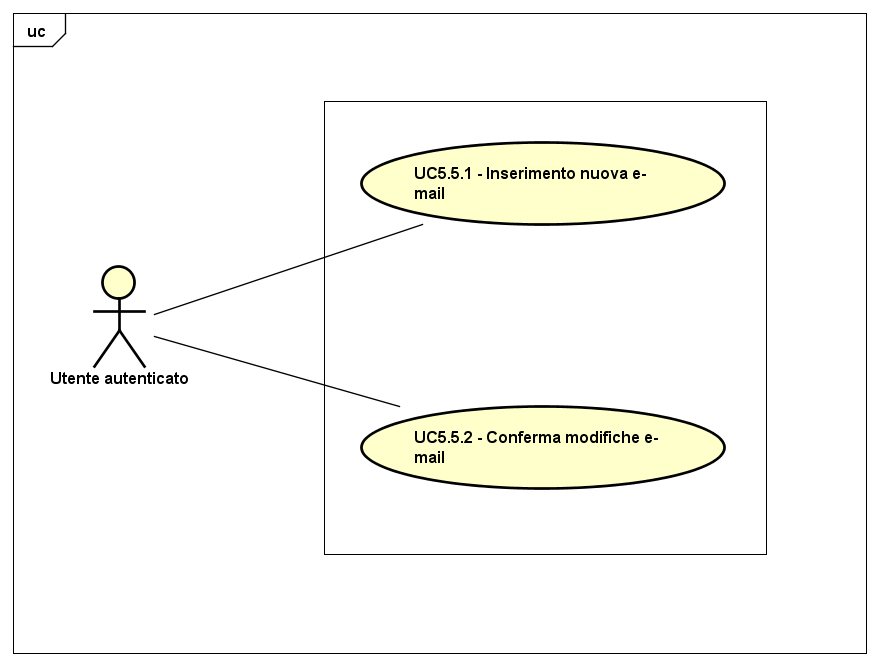
\includegraphics[scale=0.5,keepaspectratio]{UML/UC5_5.png}
	\caption{UC5.5: Modifica password}
\end{figure}

\begin{itemize}
	\item \textbf{Attori}: utente autenticato, utente autenticato pro;
	\item \textbf{Descrizione}: l'attore può modificare la propria password inserendone una nuova;
	\item \textbf{Precondizione}: il sistema visualizza l'opzione di modifica password;
	\item \textbf{Postcondizione}: il sistema ha reso persistenti le modifiche alla propria password;
	\item \textbf{Scenario principale}:
	\begin{enumerate}
		\item L'attore può inserire la propria vecchia password (UC5.5.1);
		\item L'attore può inserire una nuova password (UC5.5.2);
		\item L'attore può inserire la conferma della nuova password (UC5.5.3).
	\end{enumerate}
	\item \textbf{Scenari alternativi}: l'attore annulla le modifiche e il sistema lo riporta alla schermata di gestione del profilo utente.
\end{itemize}

\subsubsection{Caso d'uso UC5.5.1: Inserimento vecchia password}

\begin{itemize}
	\item \textbf{Attori}: utente autenticato, utente autenticato pro;
	\item \textbf{Descrizione}: l'attore può inserire la vecchia password;
	\item \textbf{Precondizione}: il sistema visualizza l'opzione per l'inserimento della vecchia password;
	\item \textbf{Postcondizione}: l'attore ha inserito la vecchia password;
	\item \textbf{Scenario principale}: l'attore inserisce la vecchia password.
\end{itemize}

\subsubsection{Caso d'uso UC5.5.2: Inserimento nuova password}

\begin{itemize}
	\item \textbf{Attori}: utente autenticato, utente autenticato pro;
	\item \textbf{Descrizione}: l'attore può inserire la nuova password;
	\item \textbf{Precondizione}: il sistema visualizza l'opzione per l'inserimento della nuova password;
	\item \textbf{Postcondizione}: l'attore inserisce la nuova password;
	\item \textbf{Scenario principale}: l'attore inserisce la nuova password.
\end{itemize}

\subsubsection{Caso d'uso UC5.5.3: Inserimento conferma nuova password}

\begin{itemize}
	\item \textbf{Attori}: utente autenticato, utente autenticato pro;
	\item \textbf{Descrizione}: l'attore può inserire la nuova password nuovamente;
	\item \textbf{Precondizione}: il sistema visualizza l'opzione per l'inserimento conferma nuova password;
	\item \textbf{Postcondizione}: l'attore inserisce nuovamente la nuova password;
	\item \textbf{Scenario principale}: l'attore inserisce nuovamente la nuova password.
\end{itemize}

\subsubsection{Caso d'uso UC5.6: Conferma modifiche profilo utente}

\begin{itemize}
	\item \textbf{Attori}: utente autenticato, utente autenticato pro;
	\item \textbf{Descrizione}: l'attore può confermare le modifiche apportare al proprio profilo utente; 
	\item \textbf{Precondizione}: il sistema visualizza l'opzione di conferma delle modifiche del profilo utente;
	\item \textbf{Postcondizione}: il sistema ha reso persistenti le modifiche al profilo utente;
	\item \textbf{Scenario principale}: l'attore conferma le modifiche apportate al proprio profilo utente;
	\item \textbf{Scenari alternativi}: l'attore annulla le modifiche e il sistema lo riporta alla schermata di gestione del profilo utente.
\end{itemize}

\subsubsection{Caso d'uso UC5.7: Visualizzazione errore conferma modifiche profilo utente}

\begin{itemize}
	\item \textbf{Attori}:  utente autenticato, utente autenticato pro;
	\item \textbf{Descrizione}: l'attore può visualizzare un messaggio d'errore se ha effettuato modifiche non permesse al proprio profilo utente;
	\item \textbf{Precondizione}: il sistema ha ricevuto dati vuoti o non validi;
	\item \textbf{Postcondizione}: il sistema mostra un messaggio d'errore;
	\item \textbf{Scenario principale}: l'attore visualizza un messaggio d'errore;
\end{itemize}

\subsubsection{Caso d'uso UC5.8: Richiesta cambio tipologia account}
\label{UC5.8}
\begin{figure}[h]
	\centering
	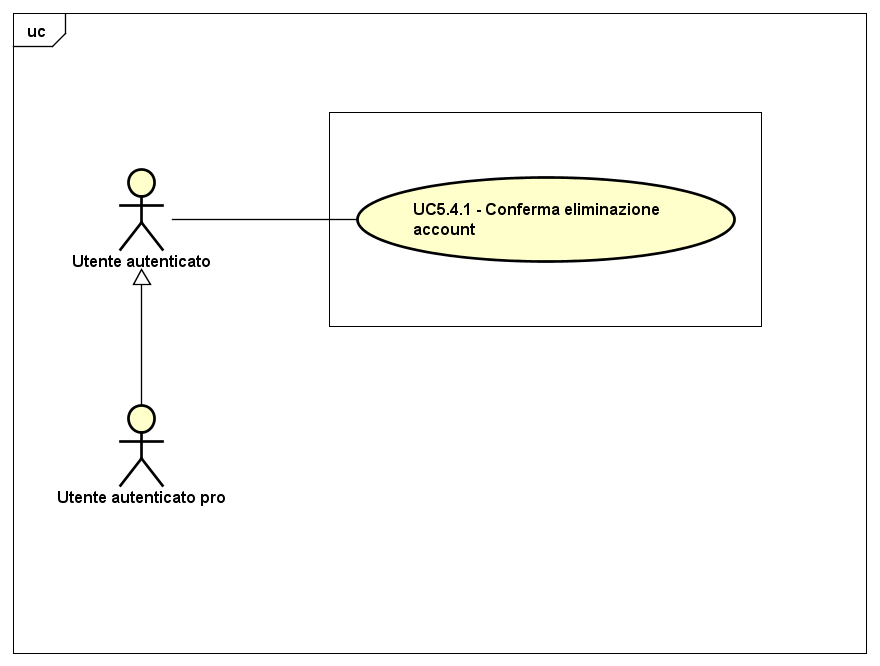
\includegraphics[scale=0.5,keepaspectratio]{UML/UC5_8.png}
	\caption{UC5.8: Richiesta cambio tipologia account}
\end{figure}

\begin{itemize}
	\item \textbf{Attori}: utente autenticato, utente autenticato pro;
	\item \textbf{Descrizione}: l'attore può richiedere di cambiare la tipologia del proprio account; 
	\item \textbf{Precondizione}: il sistema visualizza l'opzione di cambio tipologia utente;
	\item \textbf{Postcondizione}: il sistema invia la richiesta del cambio tipologia account;
	\item \textbf{Scenario principale}:
	\begin{enumerate}
		\item L'attore può selezionare il nuovo tipo di account a cui passare (UC5.8.1);
		\item L'attore può confermare l'invio della richiesta del cambio della tipologia del proprio account (UC5.8.2).
	\end{enumerate}
	\item \textbf{Scenari alternativi}: l'attore annulla le modifiche e il sistema lo riporta alla schermata di gestione del profilo utente.
\end{itemize}

\subsubsection{Caso d'uso UC5.8.1: Selezione tipologia account}

\begin{itemize}
	\item \textbf{Attori}: utente autenticato, utente autenticato pro;
	\item \textbf{Descrizione}: l'attore può selezionare una nuova tipologia di account a cui passare; se l'attore è un utente autenticato potrà scegliere di diventare un utente autenticato pro; se l'attore è un utente autenticato pro può scegliere di diventare un utente autenticato;
	\item \textbf{Precondizione}: il sistema visualizza le tipologie di account a cui passare;
	\item \textbf{Postcondizione}: l'attore ha selezionato  una nuova tipologia di account;
	\item \textbf{Scenario principale}: l'attore seleziona una tipologia di account a cui passare.
\end{itemize}

\subsubsection{Caso d'uso UC5.8.2: Invio richiesta cambio tipologia account}

\begin{itemize}
	\item \textbf{Attori}: utente autenticato, utente autenticato pro;
	\item \textbf{Descrizione}: l'attore può inviare la richiesta di passaggio alla nuova tipologia di account;
	\item \textbf{Precondizione}: il sistema visualizza l'opzione di invio richiesta cambio tipologia account;
	\item \textbf{Postcondizione}: il sistema invia la richiesta del cambio tipologia account;
	\item \textbf{Scenario principale}: l'attore invia la richiesta di cambio tipologia account.
\end{itemize}

\subsubsection{Caso d'uso UC5.9: Eliminazione account}
\label{UC5.9}
\begin{figure}[h]
	\centering
	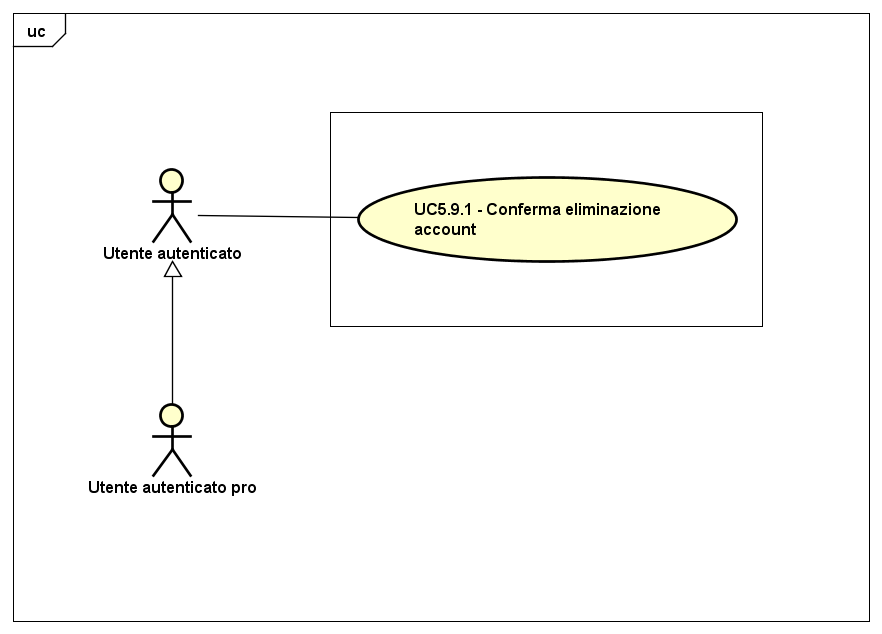
\includegraphics[scale=0.5,keepaspectratio]{UML/UC5_9.png}
	\caption{UC5.9: Eliminazione account}
\end{figure}

\begin{itemize}
	\item \textbf{Attori}: utente autenticato, utente autenticato pro;
	\item \textbf{Descrizione}: l'attore può eliminare il proprio account dal sistema; l'eliminazione dell'account comporta la cancellazione dei propri dati dal sistema; 
	\item \textbf{Precondizione}: il sistema visualizza l'opzione per l'eliminazione dell'account;
	\item \textbf{Postcondizione}: il sistema ha eliminato in maniera persistente l'account e tutti i relativi dati;
	\item \textbf{Scenario principale}: l'utente può confermare l'eliminazione del proprio account e dei relativi dati personali (UC5.9.1);
	\item \textbf{Scenari alternativi}: l'attore annulla l'eliminazione dell'account e il sistema lo riporta alla schermata di gestione del profilo utente.
\end{itemize}

\subsubsection{Caso d'uso UC5.9.1: Conferma eliminazione account}

\begin{itemize}
	\item \textbf{Attori}: utente autenticato, utente autenticato pro;
	\item \textbf{Descrizione}: l'attore può confermare la cancellazione del proprio account e dei relativi dati dal sistema;
	\item \textbf{Precondizione}: il sistema visualizza l'opzione per la conferma dell'eliminazione dell'account;
	\item \textbf{Postcondizione}: il sistema ha eliminato l'account dell'attore richiedente e tutti i relativi dati;
	\item \textbf{Scenario principale}: l'attore conferma l'eliminazione del proprio account.
\end{itemize}

\subsection{Caso d'uso UC7: Compilazione questionario selezionato}
\begin{center}
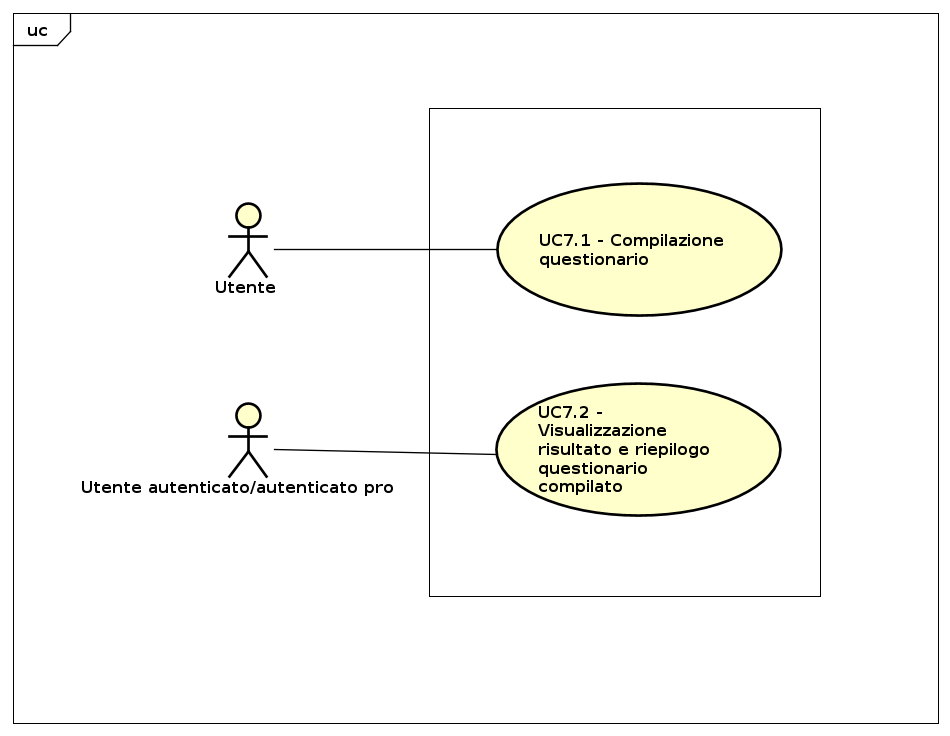
\includegraphics[scale=0.5]{UML/UC7.png}
\end{center}
\begin{itemize}
\item\textbf{Attori Principali}: Utente non autenticato, Utente autenticato, Utente autenticato pro;
\item\textbf{Descrizione}: l'utente autenticato/autenticato pro può compilare qualsiasi tipo di questionario e infine visualizzare il risultato ottenuto e il riepilogo delle risposte date. L'utente non autenticato invece può soltanto svolgere i questionari \textit{pubblici}.
\item\textbf{Precondizione}: l'utente ha selezionato un questionario;
\item\textbf{Postcondizione}: l'utente ha finito di compilare il questionario e può quindi visualizzare la valutazione finale che ha ottenuto e il riepilogo delle risposte date, se è un utente autenticato/autenticato pro;
\item\textbf{Scenario principale}:
\begin{itemize}
\item L'utente compila un questionario \textit{pubblico} (UC7.1);
\item L'utente autenticato/autenticato pro compila un questionario \textit{privato} (UC7.2);
\item L'utente autenticato/autenticato pro visualizza il risultato del questionario svolto (UC7.3).
\end{itemize}
\end{itemize}

\subsection{Caso d'uso UC7.1: Compilazione questionario pubblico}
\begin{itemize}
\item\textbf{Attori Principali}: Utente non autenticato, Utente autenticato, Utente autenticato pro;
\item\textbf{Descrizione}: -IDEA-: l'utente risponde alle domande che gli si presentano nell'ordine che preferisce spostandosi alla domanda successiva o a quella precedente ed infine conferma le risposte date;
\item\textbf{Precondizione}: l'utente ha selezionato un questionario \textit{pubblico};
\item\textbf{Postcondizione}: l'utente ha finito di compilare il questionario;
\item\textbf{Scenario principale}: -IDEA-:
\begin{itemize}
\item L'utente risponde ad una domanda (UC7.1.1);
\item L'utente passa alla domanda successiva (UC7.1.2);
\item L'utente passa alla domanda precedente (UC7.1.3);
\item L'utente conferma le risposte date alle domande (UC7.1.4);
\end{itemize}
\end{itemize}

\subsection{Caso d'uso UC7.2: Compilazione questionario privato}
\begin{center}
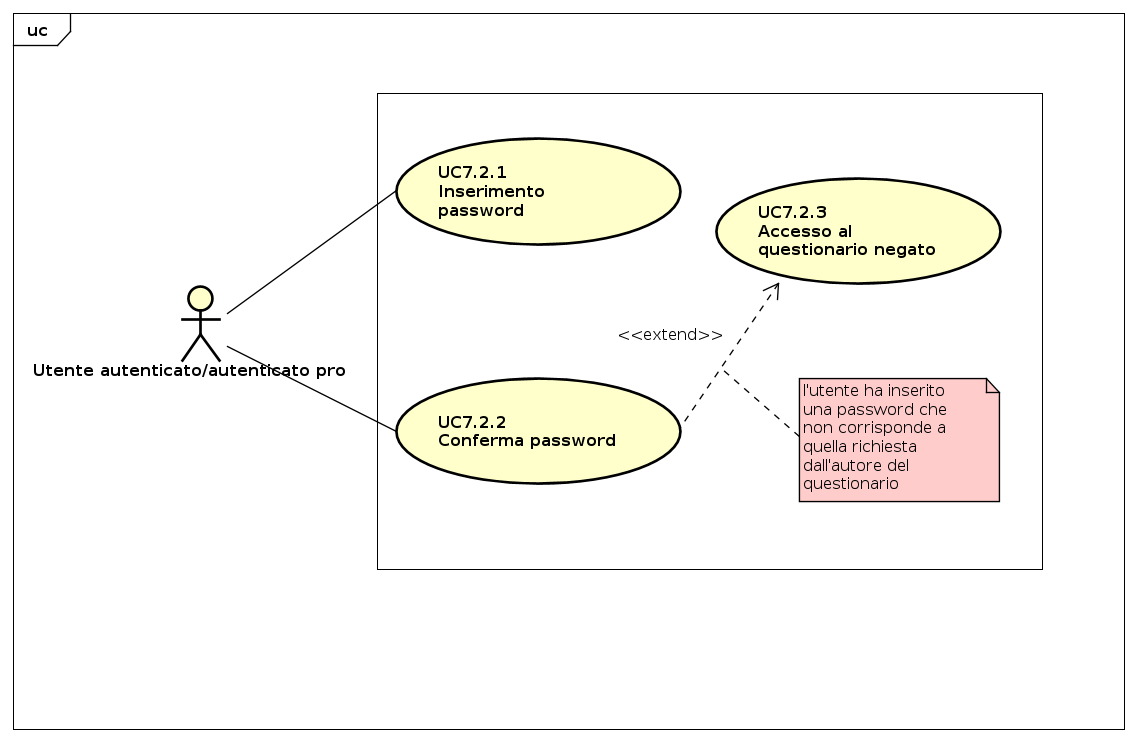
\includegraphics[scale=0.5]{UML/UC7_2.png}
\end{center}
\begin{itemize}
\item\textbf{Attori Principali}: Utente autenticato, Utente autenticato pro;
\item\textbf{Descrizione}: l'utente deve inserire la password richiesta dall'autore del questionario \textit{privato} e successivamente confermarla per poterlo compilare;
\item\textbf{Precondizione}: l'utente ha selezionato un questionario \textit{privato};
\item\textbf{Postcondizione}: l'utente ha finito di compilare il questionario;
\item\textbf{Scenario principale}:
\begin{itemize}
\item L'utente inserisce la password (UC7.2.1).
\item L'utente conferma l'inserimento della password (UC7.2.2)
\item L'utente compila il questionario (come in UC7.1)
\end{itemize}
\item\textbf{Scenario alternativo}: L'utente inserisce una password errata;
\item\textbf{Estensioni}: Accesso al questionario negato (UC7.2.3)
\end{itemize}

\subsection{Caso d'uso UC7.2.1: Inserimento password}
\begin{itemize}
\item\textbf{Attori Principali}: Utente autenticato, Utente autenticato pro;
\item\textbf{Descrizione}: l'utente per poter compilare il questionario deve inserire la password richiesta dal creatore di quest'ultimo;
\item\textbf{Precondizione}: l'utente ha selezionato un questionario \textit{privato};
\item\textbf{Postcondizione}: l'utente ha inserito la password;
\item\textbf{Scenario principale}: l'utente inserisce la password che gli consente di accedere al questionario.
\end{itemize}

\subsection{Caso d'uso UC7.2.2: Conferma password}
\begin{itemize}
\item\textbf{Attori Principali}: Utente autenticato, Utente autenticato pro;
\item\textbf{Descrizione}: l'utente conferma la password inserita per poter accedere al questionario;
\item\textbf{Precondizione}: l'utente ha inserito la password;
\item\textbf{Postcondizione}: l'utente ha confermato la password inserita;
\item\textbf{Scenario principale}: l'utente conferma la password.
\end{itemize}

\subsection{Caso d'uso UC7.2.3: Accesso al questionario negato}
\begin{itemize}
\item\textbf{Attori Principali}: Utente autenticato, Utente autenticato pro;
\item\textbf{Descrizione}: l'utente ha inserito una password che non corrisponde a quella richiesta dall'autore del questionario, generando così un errore che gli impedirà di proseguire con la compilazione del suddetto fino a quando non inserirà la password corretta;
\item\textbf{Precondizione}: l'utente ha provato a confermare una password errata;
\item\textbf{Postcondizione}: il sistema avvisa l'utente dell'errore verificatosi tramite un opportuno messaggio;
\item\textbf{Scenario principale}: l'utente visualizza il messaggio di errore relativo alla password scorretta.
\end{itemize}

\subsection{Caso d'uso UC7.3: Visualizzazione risultato questionario compilato}
\begin{itemize}
\item\textbf{Attori Principali}: Utente autenticato, Utente autenticato pro;
\item\textbf{Descrizione}: l'utente, dopo aver finito di compilare il questionario, visualizzerà una schermata contenente il riepilogo delle risposte date alle domande. Sarà possibile vedere quali di queste sono corrette e quali no e verrà inoltre data una valutazione complessiva;
\item\textbf{Precondizione}: l'utente ha finito di compilare il questionario che ha scelto di affrontare;
\item\textbf{Postcondizione}: il sistema visualizza una schermata contenente il riepilogo del questionario svolto e un voto;
\item\textbf{Scenario principale}: L'utente visualizza che voto gli è stato dato e quali domande ha sbagliato.
\end{itemize}



\newpage
\subsection{Caso d'uso UC7: Compilazione questionario}
\label{UC7}
\begin{figure}[h]
\centering
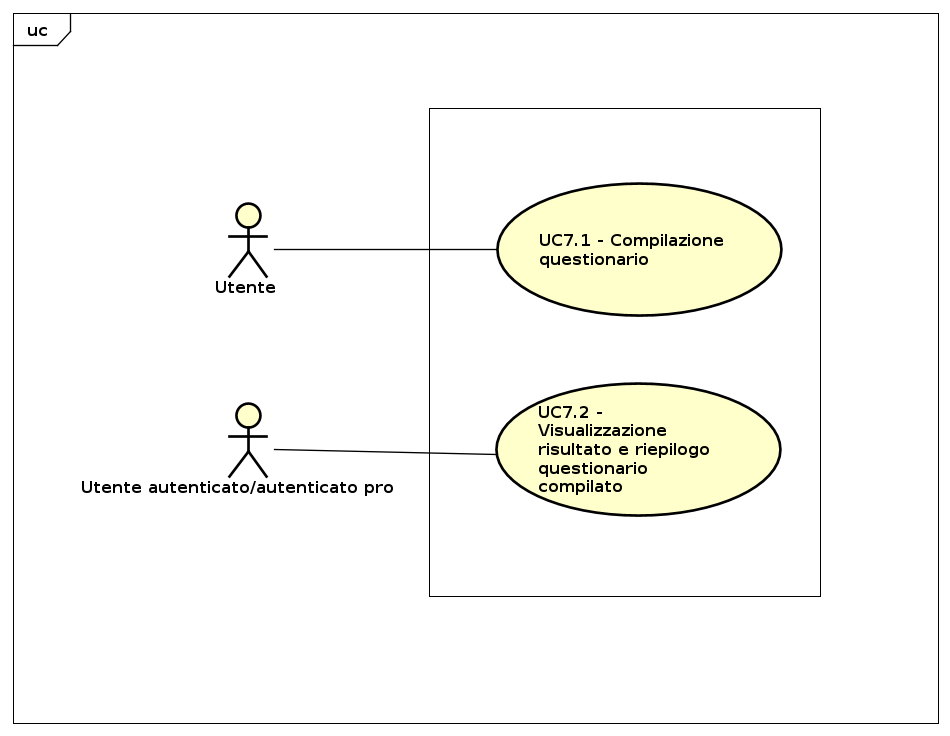
\includegraphics[scale=0.5,keepaspectratio]{UML/UC7.png}
\caption{UC7: Compilazione questionario}
\end{figure}
\FloatBarrier
\begin{itemize}
\item\textbf{Attori}: utente autenticato, utente autenticato pro;
\item\textbf{Descrizione}: l'attore che compila un questionario può rispondere alle domande che gli si presentano nell'ordine che preferisce spostandosi alla domanda successiva, a quella precedente oppure ad una a sua scelta e infine conferma le risposte date per poter visualizzare il risultato ottenuto e il riepilogo delle risposte date;
\item\textbf{Precondizione}: l'attore si è iscritto ad un questionario e l'autore del questionario ne ha abilitato la compilazione;
\item\textbf{Postcondizione}: l'attore visualizza la valutazione finale che ha ottenuto e il riepilogo delle risposte date;
\item\textbf{Scenario principale}:
\begin{itemize}
\item L'attore passa alla domanda successiva (UC7.1);
\item L'attore passa alla domanda precedente (UC7.2);
\item L'attore passa ad una domanda a sua scelta (UC7.3);
\item L'attore conferma le risposte date alle domande (UC7.4);
\item L'attore visualizza il risultato e il riepilogo del questionario svolto (UC7.5).
\end{itemize}
\item\textbf{Scenari alternativi}: nel caso in cui il questionario non è stato abilitato compare una schermata di attesa e l'attore può annullare l'operazione tornando alla schermata precedente.
\end{itemize}

\subsubsection{Caso d'uso UC7.1: Spostamento alla domanda successiva}
\label{UC7.1}
\begin{itemize}
\item\textbf{Attori}: utente autenticato, utente autenticato pro;
\item\textbf{Descrizione}: l'attore può passare alla domanda successiva;
\item\textbf{Precondizione}: l'attore sta compilando un questionario;
\item\textbf{Postcondizione}: il sistema visualizza la domanda successiva;
\item\textbf{Scenario principale}: l'attore seleziona il comando per passare alla domanda successiva.
\end{itemize}

\subsubsection{Caso d'uso UC7.2: Spostamento alla domanda precedente}
\label{UC7.2}
\begin{itemize}
\item\textbf{Attori}: utente autenticato, utente autenticato pro;
\item\textbf{Descrizione}: l'attore può passare alla domanda precedente;
\item\textbf{Precondizione}: l'attore sta compilando un questionario;
\item\textbf{Postcondizione}: il sistema visualizza la domanda precedente;
\item\textbf{Scenario principale}: l'attore seleziona il comando per passare alla domanda precedente.
\end{itemize}

\subsubsection{Caso d'uso UC7.3: Spostamento ad una domanda a scelta}
\label{UC7.3}
\begin{itemize}
\item\textbf{Attori}: utente autenticato, utente autenticato pro;
\item\textbf{Descrizione}: l'attore può passare ad una domanda a sua scelta selezionandola attraverso la tabella delle domande. Queste saranno identificate da un numero, in base all'ordine in cui sono poste all'interno del questionario, e da un colore, arancioni se è già stata data una risposta oppure grige in caso contrario;
\item\textbf{Precondizione}: l'attore sta compilando un questionario;
\item\textbf{Postcondizione}: il sistema visualizza la domanda selezionata dall'attore;
\item\textbf{Scenario principale}: l'attore seleziona una domanda a cui deve ancora rispondere o una alla quale vuole cambiare la risposta data.
\end{itemize}

\subsubsection{Caso d'uso UC7.4: Conferma risposte}
\label{UC7.4}
\begin{itemize}
\item\textbf{Attori}: utente autenticato, utente autenticato pro;
\item\textbf{Descrizione}: l'attore può confermare le domande a cui ha dato una risposta;
\item\textbf{Precondizione}: l'attore sta compilando un questionario;
\item\textbf{Postcondizione}: l'attore ha confermato le risposte date;
\item\textbf{Scenario principale}: l'attore che ha finito di rispondere a tutte le domande conferma le risposte date;
\item\textbf{Scenari alternativi}: l'attore conferma le risposte date anche se non le ha compilate tutte, accettando il fatto che queste verranno considerate sbagliate.
\end{itemize}

\subsubsection{Caso d'uso UC7.5: Visualizzazione risultato e riepilogo questionario compilato}
\label{UC7.5}
\begin{itemize}
\item\textbf{Attori}: utente autenticato, utente autenticato pro;
\item\textbf{Descrizione}: l'attore, dopo aver finito di compilare il questionario, può visualizzare una schermata contenente il riepilogo delle risposte date alle domande. Sarà possibile vedere quali di queste sono corrette e quali no e verrà inoltre data una valutazione complessiva;
\item\textbf{Precondizione}: l'attore ha finito di compilare il questionario;
\item\textbf{Postcondizione}: il sistema visualizza una schermata contenente il riepilogo del questionario svolto e un voto;
\item\textbf{Scenario principale}: l'attore visualizza che voto gli è stato dato e a quali domande ha risposto correttamente o meno.
\end{itemize}

\subsubsection{Caso d'uso UC8: Gestione dei questionari}

\newpage
\subsection{Caso d'uso UC9: Gestione dei questionari}
\label{UC9}
\begin{figure}[h]
	\centering
	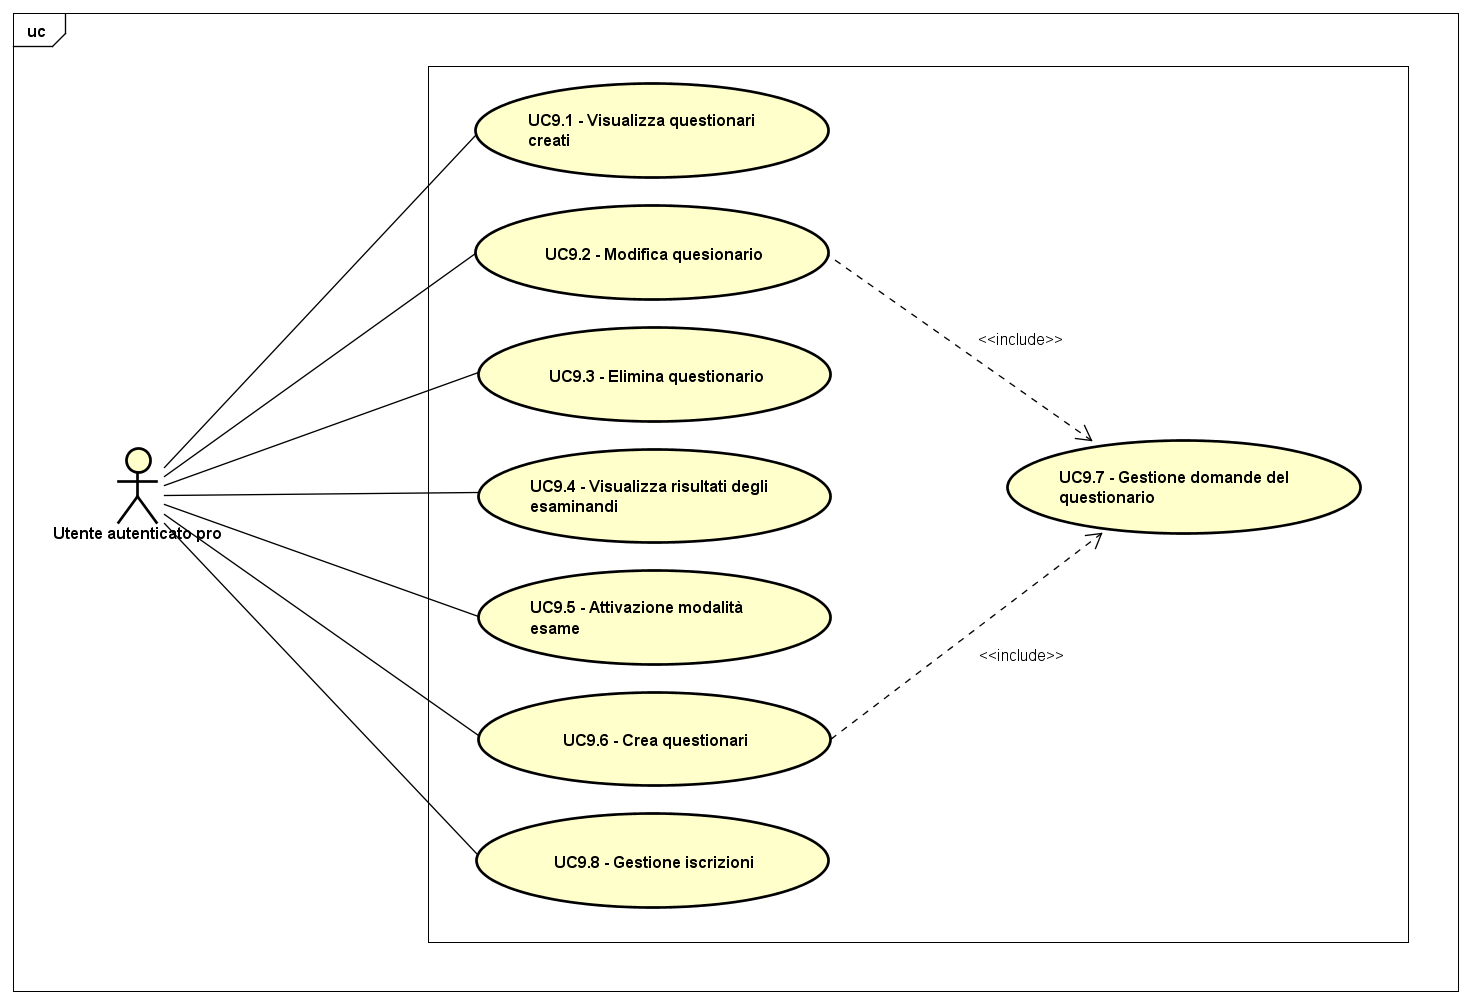
\includegraphics[scale=0.445,keepaspectratio]{UML/UC9.png}
	\caption{UC9: Gestione dei questionari}
\end{figure}
\FloatBarrier
\begin{itemize}
	\item \textbf{Attori}: \uaupro{};
	\item \textbf{Descrizione}: l'attore può modificare e/o eliminare i questionari creati da se stesso, crearne di nuovi, gestire le iscrizioni per i questionari ed infine attivare la modalità esame; 
	\item \textbf{Precondizione}: il sistema mostra la sezione della gestione dei questionari;
	\item \textbf{Postcondizione}: il sistema ha attuato le modifiche effettuate dall'attore ai propri questionari;
	\item \textbf{Scenario principale}:
		\begin{enumerate}
			\item L'attore può visualizzare i questionati creati (UC9.1);
			\item L'attore può modificare un questionario (UC9.2);
			\item L'attore può eliminare un questionario (UC9.3);
			\item L'attore può visualizzare i risultati degli esaminandi (UC9.4);
			\item L'attore può attivare la modalità esame di un questionario (UC9.5);
			\item L'attore può creare un questionario (UC9.6);
			\item L'attore può creare gestire le iscrizioni degli utenti per gli esami (UC9.8).
		\end{enumerate}
		\item \textbf{Inclusioni}: l'attore può gestire le domande di un questionario (UC9.7).		
\end{itemize}
							
	\subsubsection{Caso d'uso UC9.1: Visualizza questionari creati}
	\label{UC9.1}
	\begin{itemize}
		\item \textbf{Attori}: \uaupro{};
		\item \textbf{Descrizione}: l'attore può visualizzare i questionari da lui creati e selezionarne uno;
		\item \textbf{Precondizione}: il sistema mostra la possibilità di visualizzare i questionari creati;
		\item \textbf{Postcondizione}: l'attore visualizza i questionari da lui creato;
	\end{itemize}
	
	\subsubsection{Caso d'uso UC9.2: Modifica questionario}
	\label{UC9.2}
	\begin{figure}[h]
		\centering
	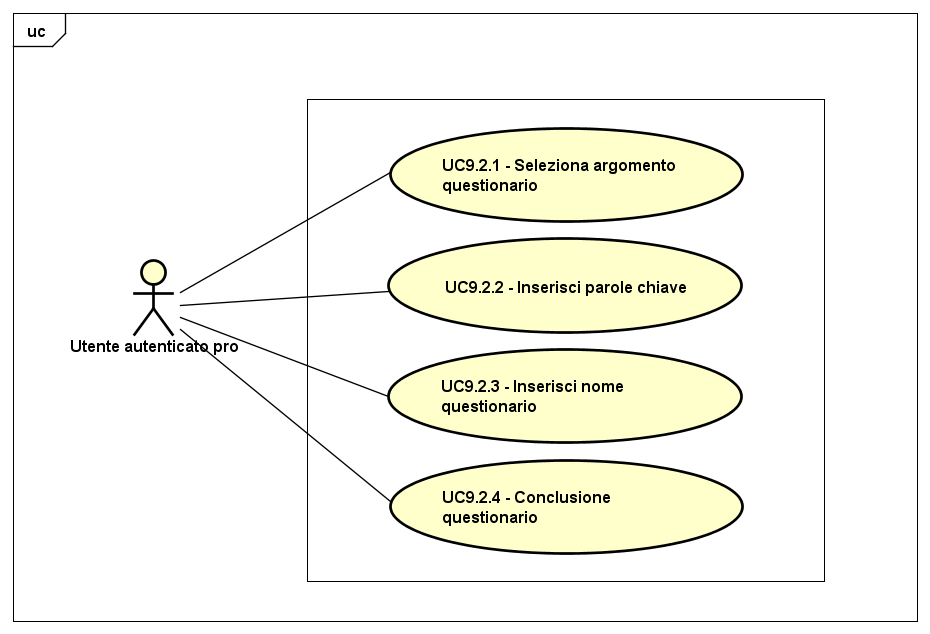
\includegraphics[scale=0.5,keepaspectratio]{UML/UC9_2.png}
		\caption{UC9.2: Modifica questionario}
	\end{figure}
	\FloatBarrier
	\begin{itemize}
		\item \textbf{Attori}: \uaupro{};
		\item \textbf{Descrizione}: l'attore può modificare il questionario selezionato;
		\item \textbf{Precondizione}: il sistema visualizza i questionari creati;
		\item \textbf{Postcondizione}: l'attore ha modificato il questionario selezionato; 
		\item \textbf{Scenario principale}:
			\begin{enumerate}
				\item L'attore può modificare il nome del questionario (UC9.2.1);
				\item L'attore può confermare le modifiche apportare (UC9.2.2).
			\end{enumerate}
	\end{itemize}
						
		\subsubsection{Caso d'uso UC9.2.1: Modifica nome questionario}
		\label{UC9.2.1}
		\begin{itemize}
			\item \textbf{Attori}: \uaupro{};
			\item \textbf{Descrizione}: l'attore può modificare il nome del questionario; 
			\item \textbf{Precondizione}: il sistema visualizza l'opzione di modifica nome questionario;
			\item \textbf{Postcondizione}: l'attore ha modificato il nome del questionario; 
			\item \textbf{Scenario principale}: l'attore modifica il nome del questionario.
		\end{itemize}
																		
		\subsubsection{Caso d'uso UC9.2.2: Conferma modifiche}
		\label{UC9.2.2}
		\begin{itemize}
			\item \textbf{Attori}: \uaupro{};
			\item \textbf{Descrizione}: l'attore può confermare le modifiche effettuate al questionario;
			\item \textbf{Precondizione}: il sistema visualizza l'opzione per confermare le modifiche effettuate;
			\item \textbf{Postcondizione}: l'attore ha confermato le modifiche effettuate;
			\item \textbf{Scenario principale}: l'attore conferma le modifiche effettuate;
			\item \textbf{Scenari alternativi}: l'attore non conferma e le modifiche fatte non vengono salvate. L'attore viene rimandato alla pagina contenente la lista dei questionari da lui creati.
		\end{itemize}
									
	\subsubsection{Caso d'uso UC9.3: Elimina questionario}
	\label{UC9.3}
	\begin{figure}[h]
		\centering
	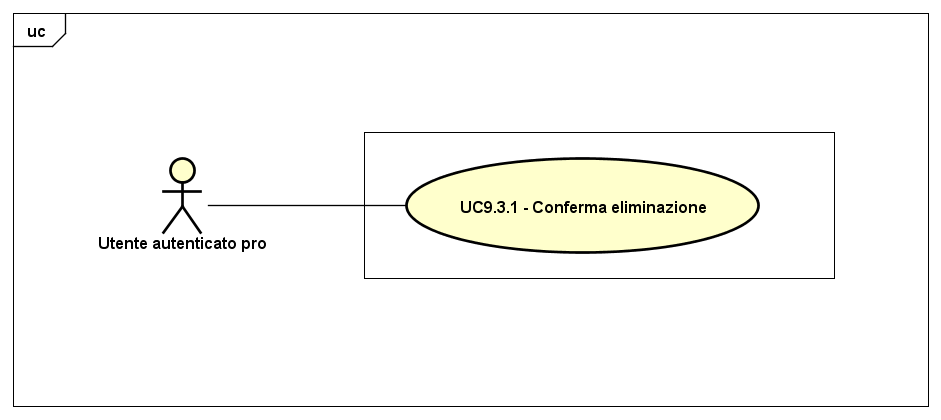
\includegraphics[scale=0.5,keepaspectratio]{UML/UC9_3.png}
		\caption{UC9.3: Elimina questionario}
	\end{figure}
	\FloatBarrier
	\begin{itemize}
		\item \textbf{Attori}: \uaupro{};
		\item \textbf{Descrizione}: l'attore può eliminare il questionario dall'archivio dei questionari;
		\item \textbf{Precondizione}: il sistema visualizza i questionari creati;
		\item \textbf{Postcondizione}: l'attore ha eliminato il questionario;
		\item \textbf{Scenario principale}: l'attore deve confermare di voler eliminare il questionario (UC9.3.1).
	\end{itemize}
	
		\subsubsection{Caso d'uso UC9.3.1: Conferma eliminazione}
		\label{UC9.3.1}
		\begin{itemize}
			\item \textbf{Attori}: \uaupro{};
			\item \textbf{Descrizione}: l'attore può confermare di voler eliminare il questionario; 
			\item \textbf{Precondizione}: il sistema visualizza l'opzione di conferma per l'eliminazione del questionario;
			\item \textbf{Postcondizione}: l'attore ha confermato di voler eliminare il questionario;
			\item \textbf{Scenario principale}: l'attore conferma di voler eliminare il questionario;
			\item \textbf{Scenari alternativi}: l'attore non conferma di voler eliminare il questionario. L'attore viene rimandato alla pagina contenente la lista dei questionari da lui creati.
		\end{itemize}
								
	\subsubsection{Caso d'uso UC9.4: Visualizza risultati degli esaminandi}
	\label{UC9.4}
	\begin{itemize}
		\item \textbf{Attori}: \uaupro{};
		\item \textbf{Descrizione}: l'attore può visualizzare le statistiche relative all'esito di un  questionario compilato dagli esaminandi;
		\item \textbf{Precondizione}: il sistema visualizza l'opzione per visualizzare i risultati degli esaminandi;
		\item \textbf{Postcondizione}: il sistema ha eseguito le opzioni scelte dall'attore;
		\item \textbf{Scenario principale}: l'attore visualizza le statistiche relative all'esito di un questionario compilato dagli esaminandi. 
	\end{itemize}
		
	\subsubsection{Caso d'uso UC9.5: Attivazione modalità esame}
	\label{UC9.5}
	\begin{itemize}
		\item \textbf{Attori}: \uaupro{};
		\item \textbf{Descrizione}: l'attore può attivare l'esame cosicché esso sia compilabile ai \uaus{};
		\item \textbf{Precondizione}: il sistema visualizza l'opzione per poter attivare la modalità esame su un determinato questionario;
		\item \textbf{Postcondizione}: il sistema ha attivato l'esame cosicché esso possa essere compilato dagli \uaus{} iscritti;
		\item \textbf{Scenario principale}: l'attore attiva l'esame cosicché esso possa essere compilato dagli \uaus{} iscritti.
	\end{itemize}
										
	\subsubsection{Caso d'uso UC9.6: Crea questionari}
	\label{UC9.6}
	\begin{figure}[h]
		\centering
	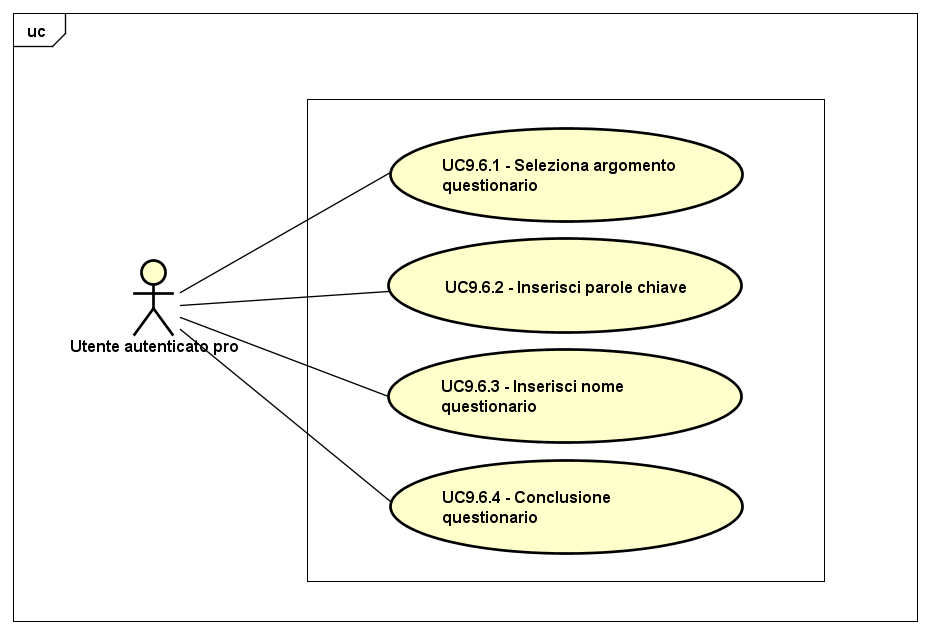
\includegraphics[scale=0.5,keepaspectratio]{UML/UC9_6.png}
		\caption{UC9.6: Crea questionari}
	\end{figure}
	\FloatBarrier
	\begin{itemize}
		\item \textbf{Attori}: \uaupro{};
		\item \textbf{Descrizione}: l'attore può creare un nuovo questionario; 
		\item \textbf{Precondizione}: il sistema visualizza l'opzione per creare nuovi questionari;
		\item \textbf{Postcondizione}: l'attore ha creato un questionario;
		\item \textbf{Scenario principale}:
			\begin{enumerate}
				\item L'attore può selezionare l'argomento del questionario (UC9.6.1);
				\item L'attore può inserire il nome del questionario (UC9.6.2);
				\item L'attore può selezionare gli argomenti del questionario (UC9.6.3);
				\item L'attore può concludere il questionario (UC9.6.4).
			\end{enumerate}
	\end{itemize}
	
		\subsubsection{Caso d'uso UC9.6.1: Seleziona argomento questionario}
		\label{UC9.6.1}
		\begin{itemize}
			\item \textbf{Attori}: \uaupro{};
			\item \textbf{Descrizione}: l'attore può selezionare l'argomento del questionario; 
			\item \textbf{Precondizione}: il sistema visualizza l'opzione per poter selezionare un argomento del questionario;
			\item \textbf{Postcondizione}: l'attore ha selezionato l'argomento del questionario;
			\item \textbf{Scenario principale}: l'attore seleziona l'argomento del questionario.
		\end{itemize}
		
		\subsubsection{Caso d'uso UC9.6.2: Inserisci parole chiave}
		\label{UC9.6.2}
		\begin{itemize}
			\item \textbf{Attori}: \uaupro{};
			\item \textbf{Descrizione}: l'attore può inserire delle parole chiave che identifichino il questionario; 
			\item \textbf{Precondizione}: il sistema visualizza l'opzione per poter inserire una parola chiave;
			\item \textbf{Postcondizione}: l'attore ha inserito delle parole chiave fino ad un massimo di quattro; 
			\item \textbf{Scenario principale}: l'attore inserisce le parole chiave che identificano il questionario.
		\end{itemize}
			
		\subsubsection{Caso d'uso UC9.6.3: Inserisci nome questionario}
		\label{UC9.6.3}
		\begin{itemize}
			\item \textbf{Attori}: \uaupro{};
			\item \textbf{Descrizione}: l'attore può inserire il nome del questionario; 
			\item \textbf{Precondizione}: il sistema visualizza l'opzione per poter inserire il nome del questionario;
			\item \textbf{Postcondizione}: l'attore ha inserito il nome del questionario; 
			\item \textbf{Scenario principale}: l'attore inserisce il nome del questionario.
		\end{itemize}
				
		\subsubsection{Caso d'uso UC9.6.4: Conclusione questionario}
		\label{UC9.6.4}
		\begin{figure}[h]
			\centering
			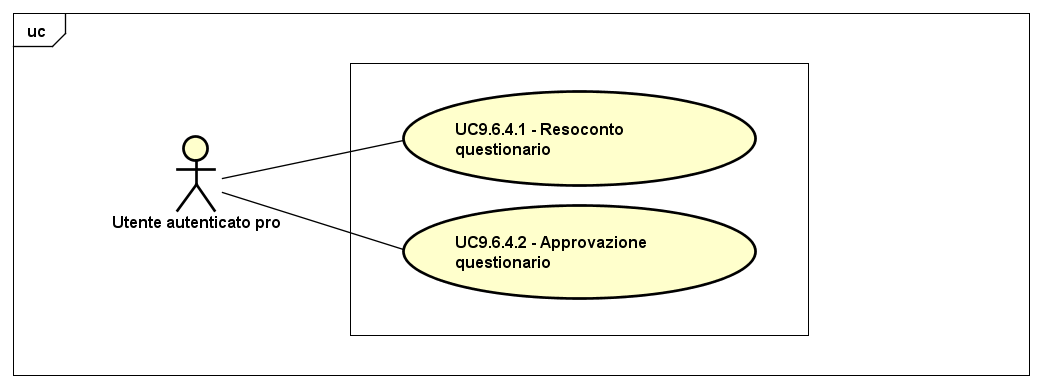
\includegraphics[scale=0.5,keepaspectratio]{UML/UC9_6_4.png}
			\caption{UC9.6.4: Conclusione questionario}
		\end{figure}
		\FloatBarrier
		\begin{itemize}
			\item \textbf{Attori}: \uaupro{}; 
			\item \textbf{Descrizione}: l'attore può smettere di inserire domande e concludere il questionario;
			\item \textbf{Precondizione}: il sistema visualizza l'opzione per poter concludere la creazione del questionario;
			\item \textbf{Postcondizione}: l'attore ha completato il questionario;
			\item \textbf{Scenario principale}: 
				\begin{enumerate}
					\item L'attore visualizza il riepilogo finale del questionario appena creato (UC9.6.4.1); 
					\item L'attore approva la creazione del questionario (UC9.6.4.2).
				\end{enumerate}
		\end{itemize}
				
			\subsubsection{Caso d'uso UC9.6.4.1: Resoconto questionario}
			\label{UC9.6.4.1}
			\begin{itemize}
				\item \textbf{Attori}: \uaupro{};
				\item \textbf{Descrizione}: l'attore può visualizzare le scelte fatte finora durante la creazione del questionario;
				\item \textbf{Precondizione}: il sistema visualizza il resoconto del questionario appena creato;
				\item \textbf{Postcondizione}: l'attore ha visualizzato le scelte fatte finora durante la creazione del questionario;
				\item \textbf{Scenario principale}: l'attore visualizza le scelte fatte finora durante la creazione del questionario.
			\end{itemize}
			
			\subsubsection{Caso d'uso UC9.6.4.2: Approvazione questionario}
			\label{UC9.6.4.2}
			\begin{itemize}
				\item \textbf{Attori}: \uaupro{};
				\item \textbf{Descrizione}: l'attore può approvare il questionario appena creato;
				\item \textbf{Precondizione}: il sistema visualizza l'opzione per poter approvare il questionario appena creato;
				\item \textbf{Postcondizione}: l'attore ha approvato il questionario;
				\item \textbf{Scenario principale}: l'attore approva il questionario;
				\item \textbf{Scenari alternativi}: l'attore non approva il questionario e quest'ultimo non viene archiviato. L'attore viene mandato alla pagina precedente.
			\end{itemize}				
	 
	 \subsubsection{Caso d'uso UC9.7: Gestione domande del questionario}
	 \label{UC9.7}
	 \begin{figure}[h]
	 	\centering
	 	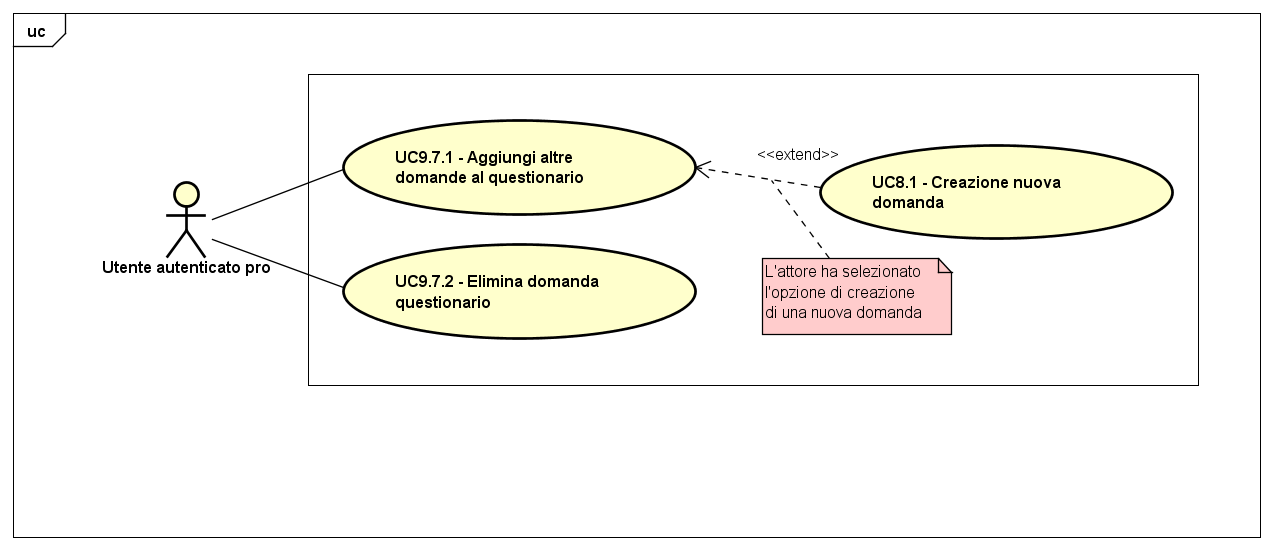
\includegraphics[scale=0.45,keepaspectratio]{UML/UC9_7.png}
	 	\caption{UC9.7: Gestione domande del questionario}
	 \end{figure}
	 \FloatBarrier
	 \begin{itemize}
	 	\item \textbf{Attori}: \uaupro{};
	 	\item \textbf{Descrizione}: l'attore può gestire le domande di un proprio questionario, aggiungendone oppure togliendone;
	 	\item \textbf{Precondizione}: il sistema visualizza l'opzione per la gestione delle domande nelle fasi di \\creazione/modifica di un questionario;
	 	\item \textbf{Postcondizione}: l'attore ha gestito le domande di un questionario;
	 	\item \textbf{Scenario principale}: 
	 	\begin{enumerate}
	 		\item L'attore aggiunge altre domande (UC9.7.1);
	 		\item L'attore elimina una domanda (UC9.7.2).
	 	\end{enumerate}
	 	\item \textbf{Estensioni}: l'attore può creare delle nuove domande per il questionario (UC8.1).		
	 \end{itemize}
	 
		 \subsubsection{Caso d'uso UC9.7.1: Aggiungi altre domande}
		 \label{UC9.7.1}
		 \begin{figure}[h]
		 	\centering
		 	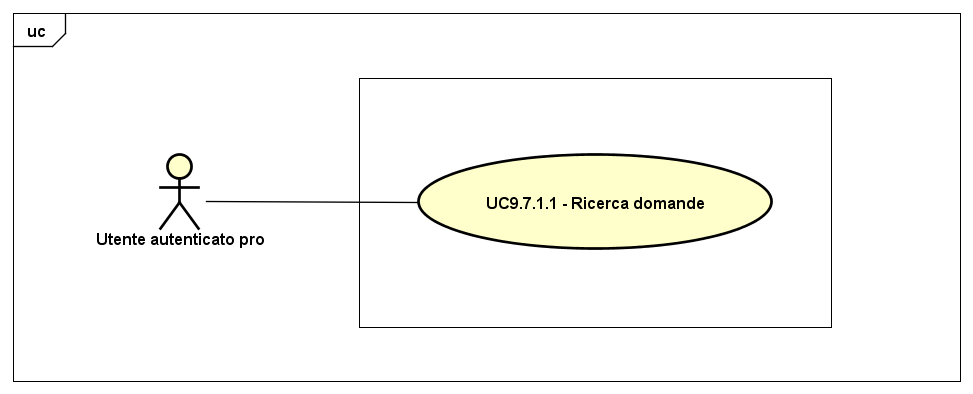
\includegraphics[scale=0.5,keepaspectratio]{UML/UC9_7_1.png}
		 	\caption{UC9.7.1: Aggiungi altre domande}
		 \end{figure}
		 \FloatBarrier
		 \begin{itemize}
		 	\item \textbf{Attori}: \uaupro{};
		 	\item \textbf{Descrizione}: l'attore può aggiungere altre domande cercando tra quelle già memorizzate nell'archivio oppure creandone una nuova; 
		 	\item \textbf{Precondizione}: il sistema visualizza l'opzione per poter aggiungere altre domande;
		 	\item \textbf{Postcondizione}: l'attore ha aggiunto nuove domande;
		 	\item \textbf{Scenario principale}: l'attore può eseguire una ricerca delle domande archiviate (UC9.7.1.1).
		 \end{itemize}
		 
			 \subsubsection{Caso d'uso UC9.7.1.1: Ricerca domande}
			 \label{UC9.7.1.1}
			 \begin{figure}[h]
			 	\centering
			 	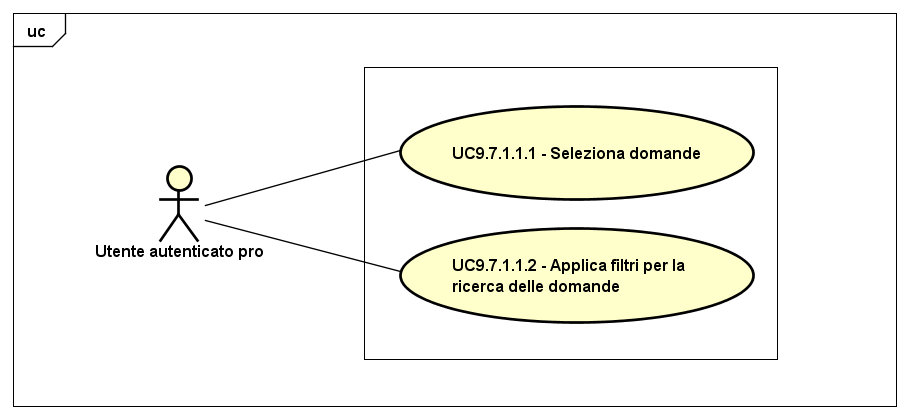
\includegraphics[scale=0.5,keepaspectratio]{UML/UC9_7_1_1.png}
			 	\caption{UC9.7.1.1: Ricerca domande}
			 \end{figure}
			 \FloatBarrier
			 \begin{itemize}
			 	\item \textbf{Attori}: \uaupro{};
			 	\item \textbf{Descrizione}: l'attore può eseguire una ricerca tra le domande archiviate; 
			 	\item \textbf{Precondizione}: il sistema visualizza l'opzione per ricercare le domande da inserire nel questionario;
			 	\item \textbf{Postcondizione}: l'attore ha ricercato tra le domande archiviate;
			 	\item \textbf{Scenario principale}:
			 	\begin{enumerate}
			 		\item L'attore può selezionare le domande (UC9.7.1.1.1); 
			 		\item L'attore può applicare dei filtri per la ricerca delle domande (UC9.7.1.1.2).
			 	\end{enumerate}
			 	\item \textbf{Estensioni}: nel caso in cui non ci sia nessun risultato dalla ricerca, all'attore viene proposta la possibilità di creare una nuova domanda (UC8.1).
			 \end{itemize}
			 
			 \subsubsection{Caso d'uso UC9.7.1.1.1: Seleziona domande}
			 \label{UC9.7.1.1.1}
			 \begin{itemize}
			 	\item \textbf{Attori}: \uaupro{};
			 	\item \textbf{Descrizione}: l'attore può selezionare le domande tra quelle ottenute dalla ricerca;
			 	\item \textbf{Precondizione}: il sistema visualizza l'opzione per poter selezionare una domanda da inserire nel questionario;
			 	\item \textbf{Postcondizione}: l'attore ha selezionato delle domande; 
			 	\item \textbf{Scenario principale}: l'attore seleziona le domande.
			 \end{itemize}
			 
			 \subsubsection{Caso d'uso UC9.7.1.1.2: Applica filtri per la ricerca delle domande}
			 \label{UC9.7.1.1.2}
			 \begin{itemize}
			 	\item \textbf{Attori}: \uaupro{};
			 	\item \textbf{Descrizione}: l'attore può applicare dei filtri per ottenere dei risultati migliori nelle ricerche: 
				 	\begin{itemize}
						\item Selezionare la difficoltà delle domande;
						\item Ordinarle per difficoltà;
						\item Ordinarle per parola chiave;
						\item Visualizzare quelle create da se stessi.
				 	\end{itemize}
			 	\item \textbf{Precondizione}: ;
			 	\item \textbf{Postcondizione}: il sistema visualizza l'opzione per poter applicare dei filtri alla ricerca; 
			 	\item \textbf{Scenario principale}: l'attore seleziona dei filtri da applicare per la ricerca.
			 \end{itemize}
		 
		 \subsubsection{Caso d'uso UC9.7.2: Elimina domanda dal questionario}
		 \label{UC9.7.2}
		 \begin{figure}[h]
		 	\centering
		 	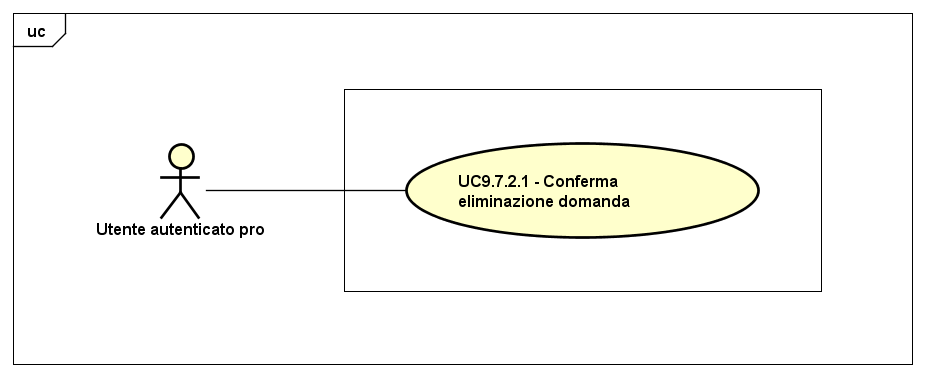
\includegraphics[scale=0.5,keepaspectratio]{UML/UC9_7_2.png}
		 	\caption{UC9.7.2: Elimina domanda dal questionario}
		 \end{figure}
		 \FloatBarrier
		 \begin{itemize}
		 	\item \textbf{Attori}: \uaupro{};
		 	\item \textbf{Descrizione}: l'attore può eliminare una domanda da un questionario;
		 	\item \textbf{Precondizione}: il sistema visualizza l'opzione per poter eliminare una domanda dal questionario;
		 	\item \textbf{Postcondizione}: l'attore ha eliminato una domanda;
		 	\item \textbf{Scenario principale}: l'attore può confermare di voler eliminare la domanda (UC9.7.2.1); 
		 	\item \textbf{Scenari alternativi}: l'attore ha cancellato tutte le domande. Deve allora inserirne almeno una, viene allora rimandato alla ricerca delle domande.
		 \end{itemize}
		 
		 \subsubsection{Caso d'uso UC9.7.2.1: Conferma eliminazione domanda}
		 \label{UC9.7.2.1}
		 \begin{itemize}
		 	\item \textbf{Attori}: \uaupro{};
		 	\item \textbf{Descrizione}: l'attore può confermare di voler eliminare la domanda;
		 	\item \textbf{Precondizione}: il sistema visualizza l'opzione per poter confermare l'eliminazione della domanda;
		 	\item \textbf{Postcondizione}: l'attore ha eliminato una domanda;
		 	\item \textbf{Scenario principale}: l'attore conferma di voler eliminare la domanda;
		 	\item \textbf{Scenari alternativi}: l'attore annulla l'eliminazione della domanda, viene allora rimandato alla schermata precedente.
		 \end{itemize}
		 
	 \subsubsection{Caso d'uso UC9.8: Gestione iscrizioni}
	 \label{UC9.8}
	 \begin{figure}[h]
	 	\centering
	 	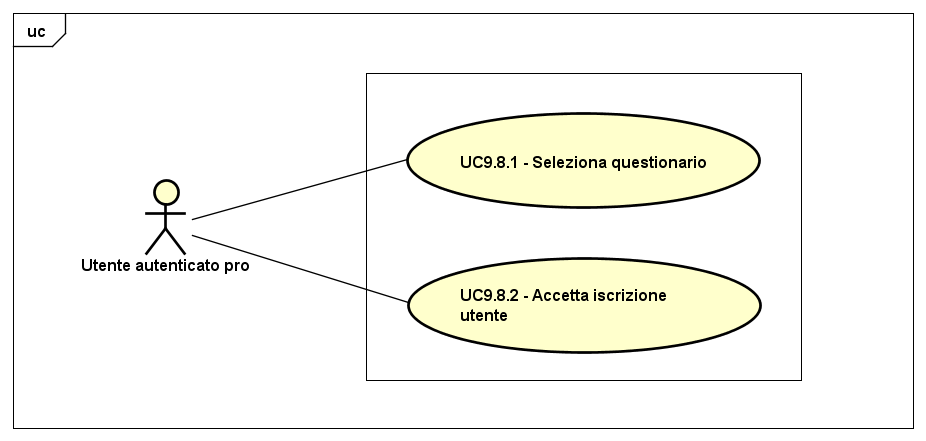
\includegraphics[scale=0.5,keepaspectratio]{UML/UC9_8.png}
	 	\caption{UC9.8: Gestione iscrizioni}
	 \end{figure}
	 \FloatBarrier
	 \begin{itemize}
	 	\item \textbf{Attori}: \uaupro{};
	 	\item \textbf{Descrizione}: l'attore può approvare le iscrizioni, per far in modo che gli utenti possano compilare un suo questionario;
	 	\item \textbf{Precondizione}: il sistema visualizza l'opzione per poter gestire le iscrizioni degli esaminandi ai questionari;
	 	\item \textbf{Postcondizione}: l'attore ha approvato la partecipazione degli utenti che vogliono prendere parte al questionario;
	 	\item \textbf{Scenario principale}: l'attore seleziona quale questionario gestire (UC9.8.1).
	 \end{itemize}
	 
		 \subsubsection{Caso d'uso UC9.8.1: Seleziona questionario}
		 \label{UC9.8.1}
		 \begin{itemize}
		 	\item \textbf{Attori}: \uaupro{};
		 	\item \textbf{Descrizione}: l'attore può selezionare il questionario del quale vuole approvare l'iscrizione degli utenti che vogliono prenderne parte. Di questo ne visualizzerà l'elenco degli utenti che hanno richiesto la partecipazione; 
		 	\item \textbf{Precondizione}: il sistema visualizza l'opzione per poter selezionare il questionario da gestire;
		 	\item \textbf{Postcondizione}: l'attore ha selezionato quale questionario gestire;
		 	\item \textbf{Scenario principale}: l'attore deve decidere quali utenti, tra quelli che vogliono partecipare, iscrivere al questionario (UC9.8.1.1).
		 \end{itemize}
		 
		 \subsubsection{Caso d'uso UC9.8.2: Accetta iscrizione utente}
		 \label{UC9.8.2}
		 \begin{itemize}
			 	\item \textbf{Attori}: \uaupro{};
			 	\item \textbf{Descrizione}: l'attore può decidere quali utenti accettare, tra quelli che vogliono partecipare al questionario; 
			 	\item \textbf{Precondizione}: il sistema visualizza il questionario selezionato dall'attore; 
			 	\item \textbf{Postcondizione}: l'attore ha approvato la partecipazione dell'\uau{} che richiede di iscriversi al questionario;
			 	\item \textbf{Scenario principale}: l'attore approva l'\uau{} che ha fatto richiesta per la partecipazione al questionario; 
			 	\item \textbf{Scenari alternativi}: nel caso in cui un \uau{} che vuole partecipare, non venga approvato, esso non avrà possibilità di accedere al questionario e ne sarà escluso.
		 \end{itemize}
			
				

\subsection{Caso d'uso UC10: Modalità allenamento}
\label{UC10}
	\begin{figure}
	\centering
	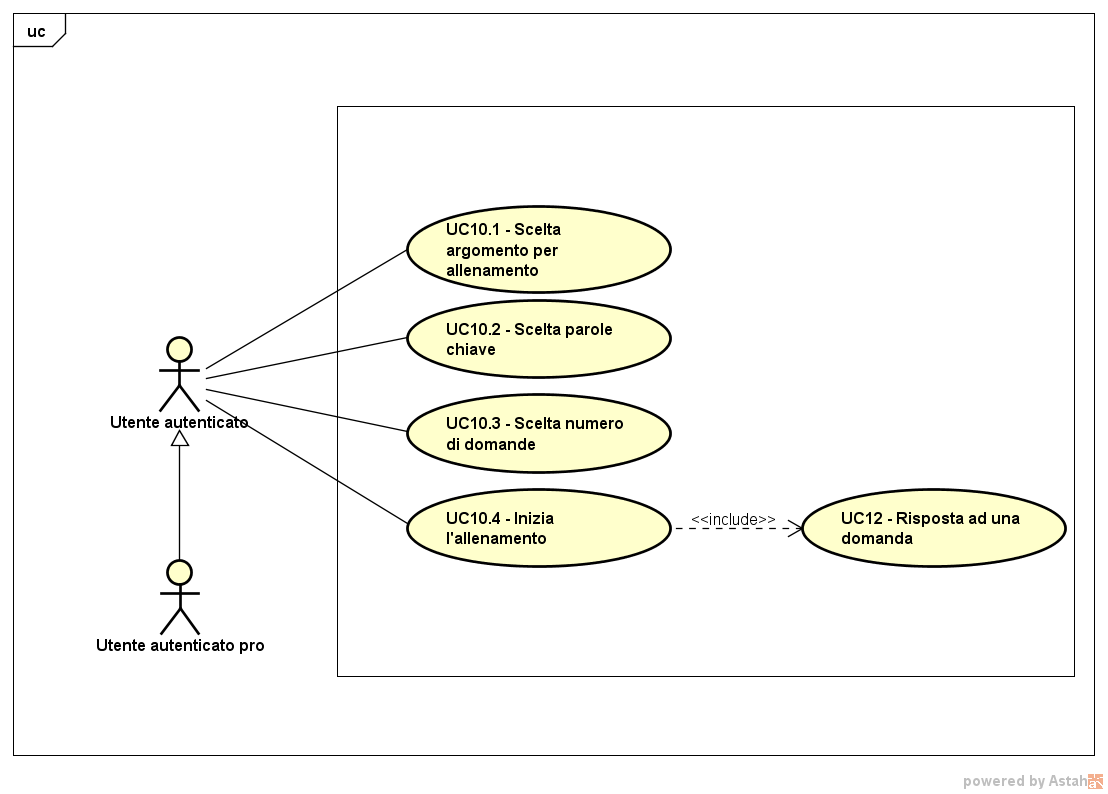
\includegraphics[scale=0.5]{UML/UC10.png}
	\caption{UC10: Modalità allenamento}
	\end{figure}
\FloatBarrier
\begin{itemize}
\item\textbf{Attori}: Utente autenticato, Utente autenticato pro;
\item\textbf{Descrizione}: gli attori possono svolgere un allenamento che consiste nel rispondere a domande che gli vengono proposte in modo dinamico. Ogni domanda può incrementare o decrementare il punteggio dell'allenamento per fare in modo che la difficoltà delle domande proposte sia sempre in linea con la competenza dell'utente sull'argomento scelto;
\item\textbf{Precondizione}: gli utenti hanno selezionato l'opzione di allenamento;
\item\textbf{Postcondizione}: gli attori hanno finito di svolgere l'allenamento e può quindi visualizzare la valutazione finale che ha ottenuto e il riepilogo delle risposte date nonché il proprio livello sugli argomenti;
\item\textbf{Scenario principale}:
	\begin{enumerate}
		\item Gli attori scelgono l'argomento per iniziare l'allenamento (UC10.1);
		\item Gli attori scelgono delle parole chiave (UC10.2);
		\item Gli attori scelgono il numero di domande che compongono l'allenamento (UC10.3);
		\item Gli attori iniziano l'allenamento (UC10.4).
	\end{enumerate}
\item \textbf{Inclusione}:
	\begin{itemize}
		\item Gli attori rispondono ad una domanda (UC12).
	\end{itemize}
\end{itemize}

\subsubsection{Caso d'uso UC10.1: Scelta argomento per l'allenamento}
	\begin{itemize}
		\item \textbf{Attori}: utente autenticato, utente autenticato pro;
		\item \textbf{Descrizione}: gli attori scelgono un macro argomento per eseguire un allenamento;
		\item \textbf{Precondizione}: gli attori scelgono di eseguire un allenamento;
		\item \textbf{Postcondizione}: gli attori hanno scelto un macro argomento per l'allenamento.
	\end{itemize}
\subsubsection{Caso d'uso UC10.2: Scelta parole chiave}
	\begin{itemize}
		\item \textbf{Attori}: utente autenticato, utente autenticato pro;
		\item \textbf{Descrizione}: gli attori scelgono delle parole chiave per filtrare in modo più dettagliato possibile l'argomento delle domande proposte per l'allenamento;
		\item \textbf{Precondizione}: gli attori hanno scelto un argomento;
		\item \textbf{Postcondizione}: gli attori hanno scelto delle parole chiavi.
	\end{itemize}
\subsubsection{Caso d'uso UC10.3: Scelta numero di domande}
	\begin{itemize}
		\item \textbf{Attori}: utente autenticato, utente autenticato pro;
		\item \textbf{Descrizione}: gli attori scelgono il numero di domande che comporranno l'allenamento, senza restrizione sul numero e ipoteticamente anche infinito;
		\item \textbf{Precondizione}: gli attori hanno scelto un argomento e scelto delle parole chiavi;
		\item \textbf{Postcondizione}: gli attori hanno scelto il numero di domande che comporranno l'allenamento.
	\end{itemize}
\subsubsection{Caso d'uso UC10.4: Inizia allenamento}
\label{UC10.4}
\begin{figure}
	\centering
	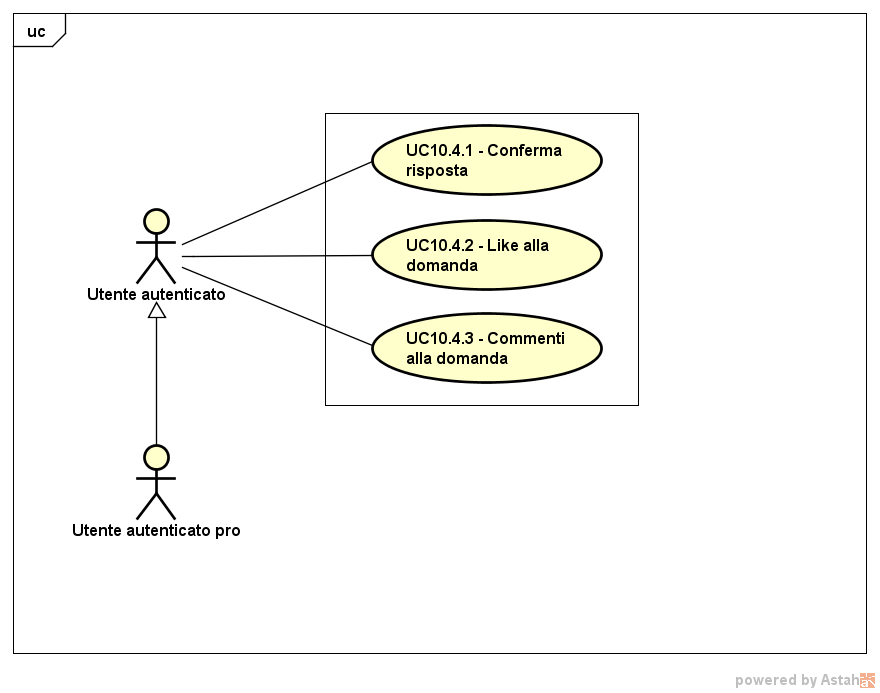
\includegraphics[scale=0.5]{UML/UC10_4.png}
	\caption{UC10.4: Inizia allenamento}
\end{figure}
\FloatBarrier
	\begin{itemize}
		\item \textbf{Attori}: utente autenticato, utente autenticato pro;
		\item \textbf{Descrizione}: gli attori iniziano l'allenamento;
		\item \textbf{Precondizione}: gli attori hanno scelto l'argomento, le parole chiave e il numero di domande;
		\item \textbf{Postcondizione}: gli attori hanno iniziato l'allenamento.
	\end{itemize}
\subsubsection{Caso d'uso UC10.4.1: Conferma risposta}
	\begin{itemize}
		\item \textbf{Attori}: utente autenticato, utente autenticato pro;
		\item \textbf{Descrizione}: gli attori confermano la risposta data;
		\item \textbf{Precondizione}: gli attori hanno risposto ad una domanda;
		\item \textbf{Postcondizione}: gli attori hanno confermato la risposta e proseguono l'allenamento.
	\end{itemize}
\subsubsection{Caso d'uso UC10.4.2: Like alla domanda}
	\begin{itemize}
		\item \textbf{Attori}: utente autenticato, utente autenticato pro;
		\item \textbf{Descrizione}: gli attori possono lasciare un like a una domanda proposta;
		\item \textbf{Precondizione}: agli attori è stata proposta una domanda;
		\item \textbf{Postcondizione}: gli attori hanno rilasciato un like alla domanda proposta.
	\end{itemize}
\subsubsection{Caso d'uso UC10.4.3: Commenti alla domanda}
\label{UC10.4.3}
\begin{figure}
	\centering
	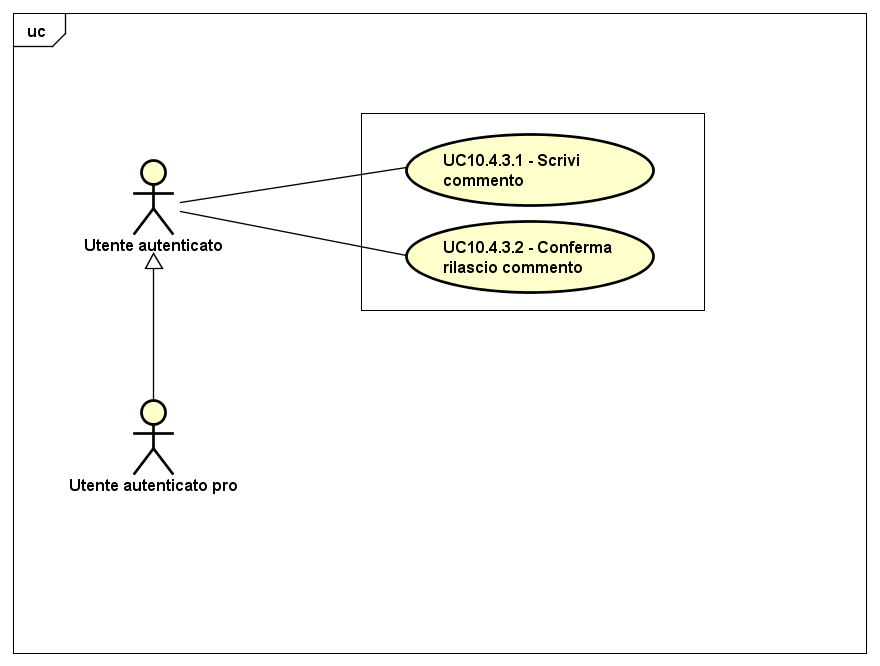
\includegraphics[scale=0.5]{UML/UC10_4_3.png}
	\caption{UC10.4.3: Commenti alla domanda}
\end{figure}
	\begin{itemize}
		\item \textbf{Attori}: utente autenticato, utente autenticato pro;
		\item \textbf{Descrizione}: gli attori possono scegliere di commentare una domanda;
		\item \textbf{Precondizione}: gli attori hanno risposto ad una domanda e visualizzano una sezione per i commenti;
		\item \textbf{Postcondizione}: gli attori hanno scelto di commentare la domanda proposta.
		\item \textbf{Scenario principale}:
			\begin{enumerate}
				\item Gli attori scrivono un commento sulla domanda (UC10.4.3.1);
				\item Gli attori confermano il rilascio del commento (UC10.4.3.2);
			\end{enumerate}
	\end{itemize}
\subsubsection{Caso d'uso UC10.4.3.1: Scrivi commento}
	\begin{itemize}
		\item \textbf{Attori}: utente autenticato, utente autenticato pro;
		\item \textbf{Descrizione}: gli attori possono scrivere il commento alla domanda proposta;
		\item \textbf{Precondizione}: gli attori hanno scelto di scrivere un commento;
		\item \textbf{Postcondizione}: gli attori hanno scritto un commento.
	\end{itemize}
\subsubsection{Caso d'uso UC10.4.3.2: Conferma rilascio commento}
	\begin{itemize}
		\item \textbf{Attori}: utente autenticato, utente autenticato pro;
		\item \textbf{Descrizione}: gli attori possono confermare il rilascio del commento scritto;
		\item \textbf{Precondizione}: gli attori hanno scritto un commento;
		\item \textbf{Postcondizione}: gli attori hanno commentato una domanda.
	\end{itemize}
\subsubsection{Caso d'uso UC10.4.4: Segnalare la domanda}
\label{UC10.4.4}
\begin{figure}
	\centering
	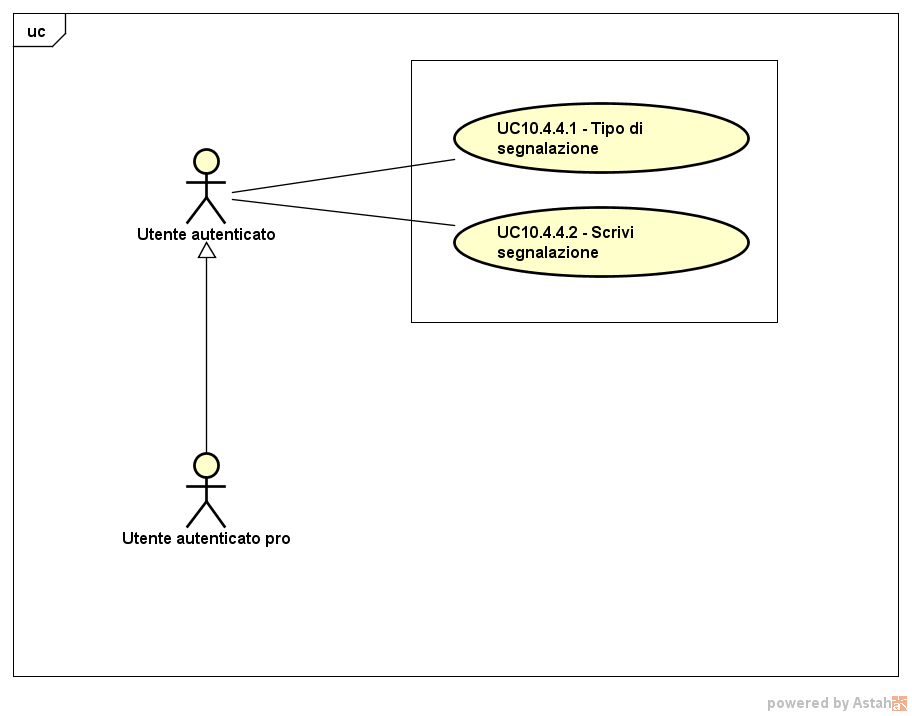
\includegraphics[scale=0.5]{UML/UC10_4_4.png}
	\caption{UC10.4.4: Segnalare una domanda}
\end{figure}
\FloatBarrier
	\begin{itemize}
		\item \textbf{Attori}: utente autenticato, utente autenticato pro;
		\item \textbf{Descrizione}: gli attori possono segnalare una domanda se ritengono che sia sbagliata, mal formata oppure contenga contenuti non appropriati;
		\item \textbf{Precondizione}: gli attori hanno visualizzato il resoconto dell'allenamento;
		\item \textbf{Postcondizione}: gli attori hanno scelto di segnalare una domanda;
				\item \textbf{Scenario principale}:
				\begin{enumerate}
					\item Gli attori scelgono il tipo di segnalazione tra quelli proposti (UC10.4.4.1);
					\item Gli attori scrivono il contenuto della segnalazione (UC10.4.4.2);
				\end{enumerate}
	\end{itemize}
\subsubsection{Caso d'uso UC10.4.4.1: Tipo di segnalazione}
	\begin{itemize}
		\item \textbf{Attori}: utente autenticato, utente autenticato pro;
		\item \textbf{Descrizione}: gli attori possono decidere il tipo di segnalazione tra quelli proposti;
		\item \textbf{Precondizione}: gli attori hanno scelto di segnalare una domanda;
		\item \textbf{Postcondizione}: gli attori hanno scelto il tipo di segnalazione.
	\end{itemize}
\subsubsection{Caso d'uso UC10.4.4.2: Scrivi segnalazione}
	\begin{itemize}
		\item \textbf{Attori}: utente autenticato, utente autenticato pro;
		\item \textbf{Descrizione}: gli attori posso scrivere un commento sulla segnalazione per approfondire la motivazione;
		\item \textbf{Precondizione}: gli attori hanno scelto di segnalare una domanda;
		\item \textbf{Postcondizione}: gli attori hanno segnalato una domanda.
	\end{itemize}
\subsubsection{Caso d'uso UC10.4.5: Avanzamento domanda successiva}
	\begin{itemize}
		\item \textbf{Attori}: utente autenticato, utente autenticato pro;
		\item \textbf{Descrizione}: gli attori possono avanzare alla domanda successiva dopo aver risposto alla domanda proposta; 
		\item \textbf{Precondizione}: gli attori hanno risposto alla domanda proposta;
		\item \textbf{Postcondizione}: gli attori visualizzano la domanda successiva.
	\end{itemize}
\subsubsection{Caso d'uso UC10.4.6: Conclusione allenamento}
	\begin{itemize}
		\item \textbf{Attori}: utente autenticato, utente autenticato pro;
		\item \textbf{Descrizione}: gli attori possono concludere l'allenamento in qualunque punto dell'allenamento;
		\item \textbf{Precondizione}: gli attori stanno eseguendo un allenamento;
		\item \textbf{Postcondizione}: gli attori hanno concluso l'allenamento e visualizzano il risultato finale e le statistiche.
	\end{itemize}

\newpage
\subsection{Caso d'uso UC11: Visualizzazione pagina utente}
\label{UC11}
\begin{figure}[h]
	\centering
	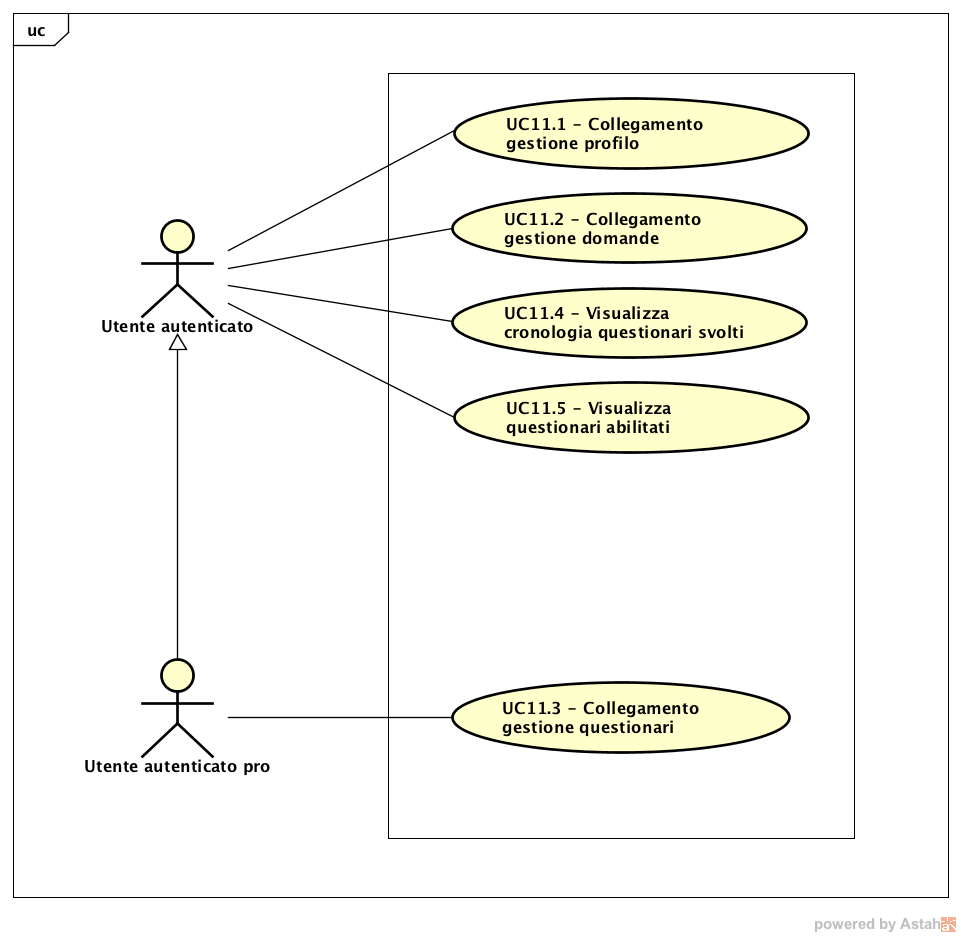
\includegraphics[scale=0.40]{UML/UC11.png}
	\caption{UC11: Gestione pagina utente}
\end{figure}

\begin{itemize}
\item\textbf{Attori}: utente autenticato, utente autenticato pro;
\item\textbf{Descrizione}: da questa pagina l'attore può: 
\begin{itemize}
	\item Visualizzare tutti i dati del proprio profilo;
	\item Visualizzare tutti i dati sugli allenamenti;
	\item Visualizzare le statistiche dei questionari svolti;
	\item Visualizzare la cronologia dei questionari svolti;
	\item Accedere alla parte del sistema che permette di modificare il profilo;
	\item Accedere alla parte del sistema che permette di aggiungere nuove domande;
	\item Accedere alla parte del sistema che permette di creare questionari.
\end{itemize}
\item\textbf{Precondizione}: il sistema mostra la pagina dell'utente;
\item\textbf{Postcondizione}: l'attore ha visualizzato i suoi dati come richiesto al sistema;
\item\textbf{Scenario principale}:
\begin{itemize}
\item L'attore può scegliere di andare alla pagina di gestione del profilo (UC11.1);
\item L'attore può scegliere di andare alla pagina di gestione delle domande (UC11.2);  
\item L'attore, solo l'\uaupro{} in questo caso, può scegliere di andare alla pagina di gestione dei questionari (UC11.3);
\item L'attore può scegliere di andare alla pagina di visualizzazione della cronologia dei questionari svolti (UC11.4);
\item L'attore può scegliere di andare alla pagina di visualizzazione dei questionari abilitati (UC11.5);
\item L'attore può scegliere di andare alla pagina principale (UC11.6);
\item L'attore visualizza il numero di allenamenti svolti (UC11.7);
\item L'attore visualizza la classifica degli argomenti scelti negli allenamenti (UC11.8);
\item L'attore visualizza il proprio livello attuale (UC11.9);
\item L'attore visualizza il numero di domande risposte in modo esatto (UC11.10);
\item L'attore visualizza il numero di domande risposte in modo sbagliato (UC11.11);
\item L'attore visualizza il proprio nome utente (UC11.12);
\item L'attore visualizza la propria immagine profilo (UC11.13).
\end{itemize}
\item\textbf{Inclusioni}: l'attore può compilare un questionario (UC7).
\end{itemize}

\subsubsection{Caso d'uso UC11.1: Collegamento gestione profilo}
\begin{itemize}
\item\textbf{Attori}: utente autenticato, utente autenticato pro;
\item\textbf{Descrizione}: l'attore viene portato nella pagina di gestione del profilo dove può modificare liberamente tutti i suoi dati;
\item\textbf{Precondizione}: il sistema mostra la pagina dell'utente;
\item\textbf{Postcondizione}: il sistema visualizza la pagina di gestione del profilo;
\item\textbf{Scenario principale}: l'attore si trova nella pagina di gestione del profilo e potrà attuare tutte le modifiche desiderate.
\end{itemize}

\subsubsection{Caso d'uso UC11.2: Collegamento gestione delle domande}
\begin{itemize}
\item\textbf{Attori}: utente autenticato, utente autenticato pro;
\item\textbf{Descrizione}: l'attore viene portato nella pagina di gestione delle domande dove può inserire o modificare le sue domande;
\item\textbf{Precondizione}: il sistema mostra la pagina dell'utente;

\item\textbf{Postcondizione}: il sistema visualizza la pagina di gestione delle domande;
\item\textbf{Scenario principale}: l'attore si trova nella pagina di gestione delle domande e potrà attuare tutte le modifiche desiderate.
\end{itemize}

\subsubsection{Caso d'uso UC11.3: Collegamento gestione questionari}
\begin{itemize}
\item\textbf{Attori}: utente autenticato, utente autenticato pro;
\item\textbf{Descrizione}: l'attore viene portato nella pagina di gestione dei questionari dove può compiere tutte le azioni possibili sui questionari;
\item\textbf{Precondizione}:il sistema mostra la pagina dell'utente;
\item\textbf{Postcondizione}: il sistema visualizza la pagina di gestione dei questionari;
\item\textbf{Scenario principale}: l'attore si trova nella pagina di gestione dei questionari e potrà attuare tutte le modifiche desiderate.
\end{itemize}

\subsubsection{Caso d'uso UC11.4: Visualizzazione cronologia questionari svolti}
\label{UC11.4}
\begin{figure}[h]
	\centering
	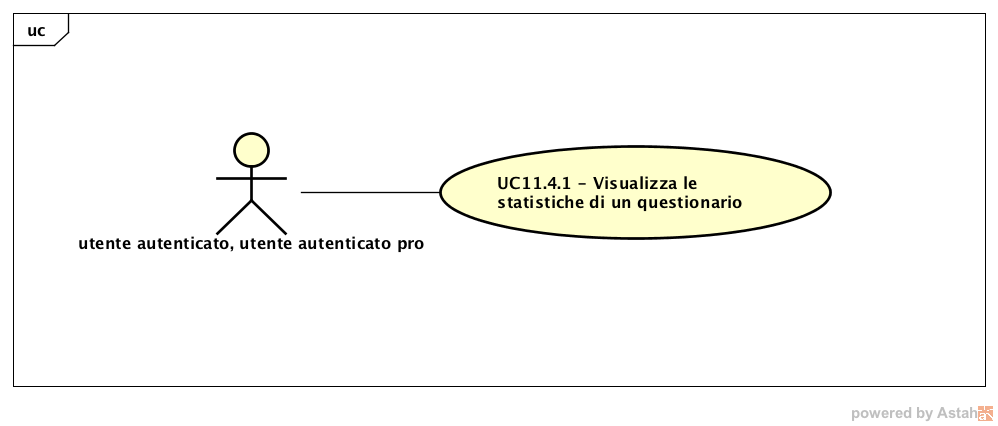
\includegraphics[scale=0.5]{UML/UC11_4.png}
	\caption{UC11.4: Visualizzazione cronologia questionari svolti}
\end{figure}
\begin{itemize}
\item\textbf{Attori}: utente autenticato, utente autenticato pro;
\item\textbf{Descrizione}: il sistema mostra la pagina dell'utente;
\item\textbf{Precondizione}: l'attore si trova nella propria pagina utente e ha compilato almeno un questionario;
\item\textbf{Postcondizione}: il sistema visualizza la cronologia dei questionari;
\item\textbf{Scenario principale}: l'attore può visualizzare le statistiche di un questionario (UC11.4.1).
\end{itemize}

\subsubsection{Caso d'uso UC11.4.1: Selezione e visualizzazione delle statistiche di un questionario scelto}
\begin{itemize}
\item\textbf{Attori}: utente autenticato, utente autenticato pro;
\item\textbf{Descrizione}: l'attore può selezionare un questionario fra quelli presenti nella cronologia e quindi visualizzarne le statistiche;
\item\textbf{Precondizione}: il sistema mostra all'attore tutti i questionari da lui svolti;
\item\textbf{Postcondizione}: il sistema ha mostrato all'attore le statistiche del questionario selezionato;
\item\textbf{Scenario principale}: l'attore si trova nella pagina dedicata alla visualizzazione delle statistiche di un particolare questionario da lui scelto.
\end{itemize}

\subsubsection{Caso d'uso UC11.5: Visualizzazione questionari abilitati}
\label{UC11.5}
\begin{figure}[h]
	\centering
	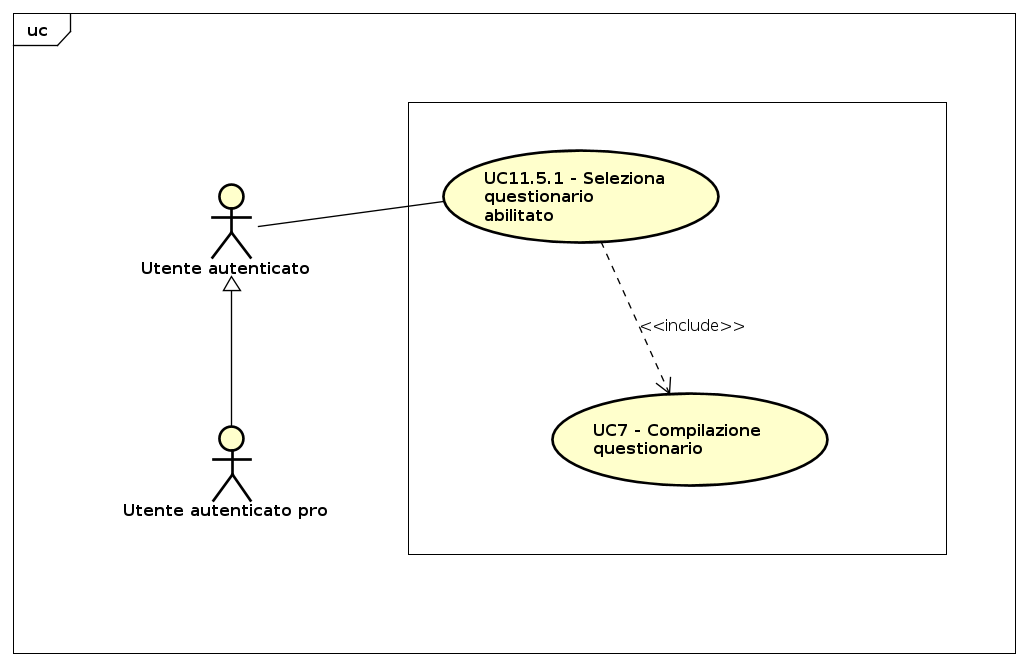
\includegraphics[scale=0.5]{UML/UC11_5.png}
	\caption{UC11.5: Visualizza questionari abilitati}
\end{figure}
\begin{itemize}
\item\textbf{Attori}: utente autenticato, utente autenticato pro;
\item\textbf{Descrizione}: l'attore può visualizzare la lista dei questionari a cui è stato abilitato da parte dell'utente autenticato pro proprietario del questionario.
\item\textbf{Precondizione}: il sistema mostra all'attore la propria pagina utente;
\item\textbf{Postcondizione}: il sistema ha mostrato all'attore tutti i questionari a cui è stato abilitato;
\item\textbf{Scenario principale}: l'attore può selezionare un questionario abilitato (UC11.5.1).
\end{itemize}

\subsubsection{Caso d'uso UC11.5.1: Seleziona questionario abilitato}
\begin{itemize}
\item\textbf{Attori}: utente autenticato, utente autenticato pro;
\item\textbf{Descrizione}: l'attore può selezionare un questionario a cui è stato abilitato e compilarlo;
\item\textbf{Precondizione}: il sistema mostra la pagina di tutti i questionari a cui l'utente è stato abilitato;
\item\textbf{Postcondizione}: l'attore ha selezionato un questionario a cui è stato abilitato;
\item\textbf{Scenario principale}: l'attore seleziona un questionario a cui è stato abilitato;
\item \textbf{Estensioni}: l'utente può compilare un questionario (UC7).
\end{itemize}

\subsubsection{Caso d'uso UC11.6: Collegamento Homepage}
\begin{itemize}
\item\textbf{Attori}: utente autenticato, utente autenticato pro;
\item\textbf{Descrizione}: l'attore può tornare alla pagina iniziale;
\item\textbf{Precondizione}: il sistema mostra la pagina dell'utente;
\item\textbf{Postcondizione}: il sistema visualizza la pagina iniziale;
\item\textbf{Scenario principale}: l'attore seleziona l'opzione per andare nella pagina iniziale.
\end{itemize}

\subsubsection{Caso d'uso UC11.7: Visualizzazione del proprio username}
\begin{itemize}
	\item\textbf{Attori}: utente autenticato, utente autenticato pro;
	\item\textbf{Descrizione}: l'attore visualizza il proprio username;
	\item\textbf{Precondizione}: il sistema visualizza la pagina utente;
	\item\textbf{Postcondizione}: il sistema visualizza l'username dell'utente;
	\item\textbf{Scenario principale}: l'attore visualizza il proprio nome utente;
\end{itemize}

\subsubsection{Caso d'uso UC11.8: Visualizzazione della propria immagine profilo }
\begin{itemize}
	\item\textbf{Attori}: utente autenticato, utente autenticato pro;
	\item\textbf{Descrizione}: l'attore visualizza la propria immagine profilo;
	\item\textbf{Precondizione}: il sistema visualizza la pagina utente;
	\item\textbf{Postcondizione}: il sistema visualizza l'immagine profilo dell'utente;
	\item\textbf{Scenario principale}: l'attore visualizza la propria immagine profilo;
\end{itemize}

\subsubsection{Caso d'uso UC11.9: Visualizzazione del proprio livello attuale }
\begin{itemize}
	\item\textbf{Attori}: utente autenticato, utente autenticato pro;
	\item\textbf{Descrizione}: l'attore visualizza il proprio livello attuale;
	\item\textbf{Precondizione}: il sistema visualizza la pagina utente;
	\item\textbf{Postcondizione}: il sistema visualizza il livello attuale dell'utente;
	\item\textbf{Scenario principale}: l'attore visualizza il proprio livello attuale.
\end{itemize}

\subsubsection{Caso d'uso UC11.10: Visualizzazione numero di allenamenti svolti}
\begin{itemize}
	\item\textbf{Attori}: utente autenticato, utente autenticato pro;
	\item\textbf{Descrizione}: l'attore visualizza il numero di allenamenti svolti;
	\item\textbf{Precondizione}: il sistema mostra la pagina dell'utente;
	\item\textbf{Postcondizione}: il sistema visualizza il numero di allenamenti svolti;
	\item\textbf{Scenario principale}: l'attore visualizza il numero di allenamenti svolti.
\end{itemize}

\subsubsection{Caso d'uso UC11.11: Visualizzazione della classifica degli argomenti scelti negli allenamenti }
\begin{itemize}
	\item\textbf{Attori}: utente autenticato, utente autenticato pro;
	\item\textbf{Descrizione}: l'attore visualizza la classifica degli argomenti scelti negli allenamenti;
	\item\textbf{Precondizione}: il sistema visualizza la pagina dell'utente;
	\item\textbf{Postcondizione}: il sistema visualizza la classifica degli argomenti scelti negli allenamenti;
	\item\textbf{Scenario principale}: l'attore visualizza la classifica degli argomenti scelti negli allenamenti.
\end{itemize}

\subsubsection{Caso d'uso UC11.12: Visualizzazione del numero di domande risposte in modo esatto}
\begin{itemize}
	\item\textbf{Attori}: utente autenticato, utente autenticato pro;
	\item\textbf{Descrizione}: l'attore visualizza il numero di domande risposte in modo corretto;
	\item\textbf{Precondizione}: il sistema visualizza la pagina utente;
	\item\textbf{Postcondizione}: il sistema visualizza il numero di domande risposte in modo esatto dall'utente;
	\item\textbf{Scenario principale}: l'attore visualizza il numero di domande risposte in modo corretto.
\end{itemize}

\subsubsection{Caso d'uso UC11.13: Visualizzazione del numero di domande risposte in modo sbagliato }
\begin{itemize}
	\item\textbf{Attori}: utente autenticato, utente autenticato pro;
	\item\textbf{Descrizione}: l'attore visualizza il numero di domande risposte in modo sbagliato;
	\item\textbf{Precondizione}: il sistema visualizza la pagina utente;
	\item\textbf{Postcondizione}: il sistema visualizza il numero di domande risposte in modo sbagliato dall'utente;
	\item\textbf{Scenario principale}: l'attore visualizza il numero di domande risposte in modo sbagliato.
\end{itemize}

\newpage
\subsection{Caso d'uso UC12: Risposta ad una domanda}
\label{UC12}
\begin{figure}[h]
	\centering
	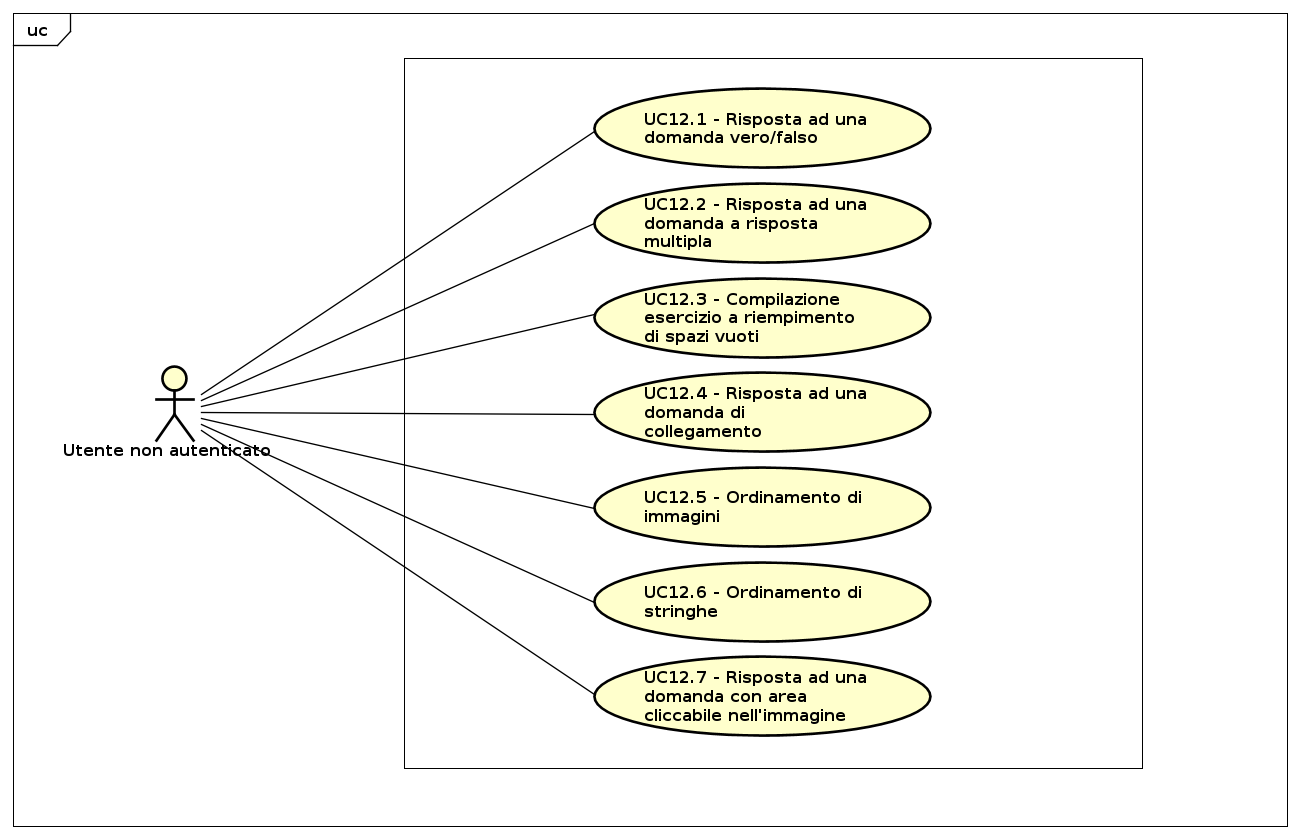
\includegraphics[scale=0.5]{UML/UC12.png}
	\caption{UC12: Risposta ad una domanda}
\end{figure}

\begin{itemize}
\item \textbf{Attori}: utente autenticato, utente autenticato pro;
\item \textbf{Descrizione}: l'attore può rispondere alla domanda che viene visualizzata selezionando una o più risposte proposte, riempiendo gli spazi vuoti, ordinando le risposte oppure associando due voci;
\item \textbf{Precondizione}: l'attore visualizza la domanda e le possibili risposte;
\item \textbf{Postcondizione}: l'attore ha selezionato una o più risposte;
\item \textbf{Scenario principale}: si verifica uno dei seguenti scenari:
\begin{enumerate}
	\item L'attore risponde ad una domanda vero/falso (UC12.1);
	\item L'attore risponde ad una domanda con risposte multiple (UC12.2);
	\item L'attore compila un esercizio riempiendo gli spazi vuoti (UC12.3);
	\item L'attore associa le voci della colonna di sinistra con quelle della colonna di destra (UC12.4);
	\item L'attore ordina le immagini secondo il criterio richiesto dalla domanda (UC12.5);
	\item L'attore ordina le stringhe secondo il criterio richiesto dalla domanda (UC12.6);
	\item L'attore risponde alla domanda selezionando un'area cliccabile (UC12.7). 
\end{enumerate}
\end{itemize}

\subsubsection{Caso d'uso UC12.1: Risposta ad una domanda vero/falso}
\begin{itemize}
\item \textbf{Attori}: utente autenticato, utente autenticato pro;
\item \textbf{Descrizione}: l'attore può selezionare una risposta alla domanda vero/falso;
\item \textbf{Precondizione}: l'attore visualizza la domanda vero/falso;
\item \textbf{Postcondizione}: l'attore ha risposto alla domanda vero/falso;
\item \textbf{Scenario principale}: l'attore seleziona una risposta alla domanda vero/falso.
\end{itemize}

\subsubsection{Caso d'uso UC12.2: Risposta ad una domanda a risposta multipla}
\begin{itemize}
\item \textbf{Attori}: utente autenticato, utente autenticato pro;
\item \textbf{Descrizione}: l'attore può selezionare una o più risposte alla domanda a risposta multipla;
\item \textbf{Precondizione}: l'attore visualizza la domanda a risposta multipla;
\item \textbf{Postcondizione}: l'attore ha risposto alla domanda a risposta multipla;
\item \textbf{Scenario principale}: l'attore seleziona una o più risposte alla domanda a risposta multipla.
\end{itemize}

\subsubsection{Caso d'uso UC12.3: Compilazione esercizio di riempimento degli spazi vuoti}
\label{UC12.3}
\begin{figure}[h]
	\centering
	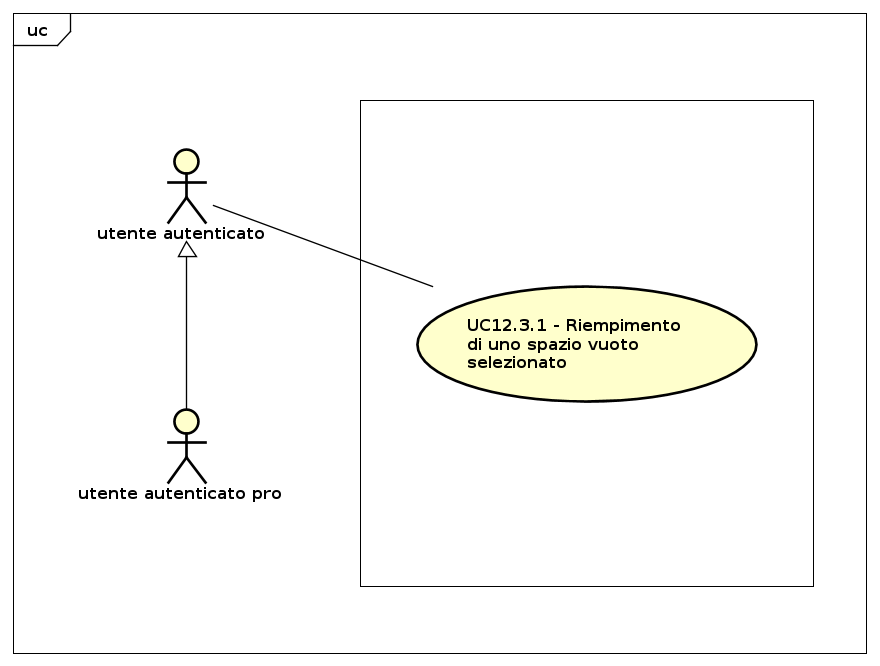
\includegraphics[scale=0.5]{UML/UC12_3.png}
	\caption{UC12.3: Compilazione esercizio di riempimento degli spazi vuoti}
\end{figure}
\begin{itemize}
\item \textbf{Attori}: utente autenticato, utente autenticato pro;
\item \textbf{Descrizione}: l'attore può compilare l'esercizio riempiendone gli spazi;
\item \textbf{Precondizione}: l'attore visualizza l'esercizio di riempimento degli spazi vuoti;
\item \textbf{Postcondizione}: l'attore ha compilato l'esercizio riempiendone gli spazi;
\item \textbf{Scenario principale}: l'attore compila l'esercizio riempiendone gli spazi  (UC12.3.1).
\end{itemize}

\subsubsection{Caso d'uso UC12.3.1: Riempimento di uno spazio vuoto selezionato}
\begin{itemize}
\item \textbf{Attori}: utente autenticato, utente autenticato pro;
\item \textbf{Descrizione}: l'attore può riempire o modificare lo spazio selezionato;
\item \textbf{Precondizione}: l'attore ha selezionato uno spazio;
\item \textbf{Postcondizione}: l'attore ha riempito lo spazio selezionato;
\item \textbf{Scenario principale}: l'attore riempie o modifica lo spazio selezionato;
\item \textbf{Scenario alternativo}: l'attore seleziona un altro spazio per riempirlo o modificarlo. 
\end{itemize}

\subsubsection{Caso d'uso UC12.4: Risposta ad una domanda di collegamento}
\begin{figure}[h]
	\centering
	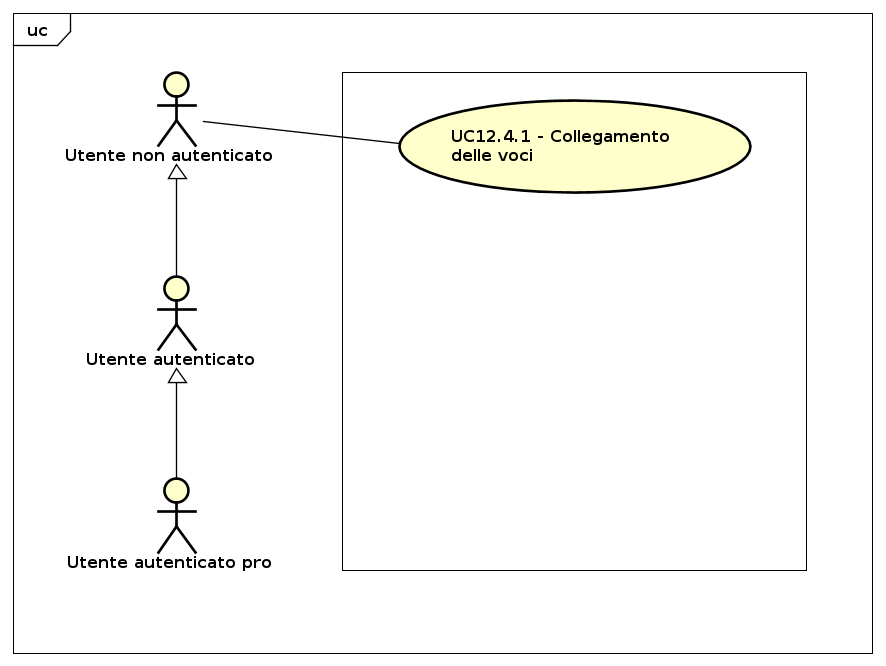
\includegraphics[scale=0.5]{UML/UC12_4.png}
	\caption{UC12.4: Risposta ad una domanda di collegamento}
\end{figure}
\begin{itemize}
\item \textbf{Attori}: utente autenticato, utente autenticato pro;
\item \textbf{Descrizione}: l'attore può collegare le voci della colonna di sinistra con le voci della colonna di destra;
\item \textbf{Precondizione}: l'attore visualizza la domanda di collegamento;
\item \textbf{Postcondizione}: l'attore ha collegato le voci della colonna di sinistra con le voci della colonna di destra;
\item \textbf{Scenario principale}: l'attore collega le voci della colonna di sinistra con le voci della colonna di destra (UC12.4.1).
\end{itemize}

\newpage
\subsubsection{Caso d'uso UC12.4.1: Collegamento delle voci}
\label{UC12.4.1}
\begin{figure}[h]
	\centering
	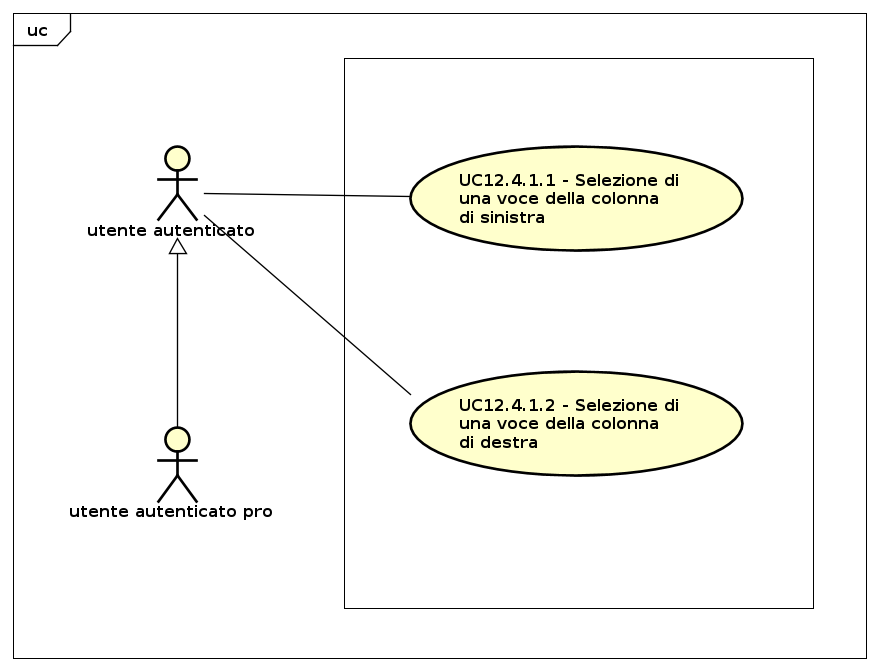
\includegraphics[scale=0.5]{UML/UC12_4_1.png}
	\caption{UC12.4.1: Collegamento delle voci}
\end{figure}
\begin{itemize}
\item \textbf{Attori}: utente autenticato, utente autenticato pro;
\item \textbf{Descrizione}: l'attore può selezionare una voce della colonna di sinistra/destra e successivamente selezionare una voce della colonna di destra/sinistra per associarle;
\item \textbf{Precondizione}: l'attore visualizza le colonne con le voci da associare;
\item \textbf{Postcondizione}: l'attore ha associato due voci;
\item \textbf{Scenario principale}: l'attore seleziona una voce della colonna di sinistra/destra (UC12.4.1.1)/(UC12.4.1.2) e successivamente seleziona una voce della colonna di destra/sinistra per associarle.
\end{itemize}

\subsubsection{Caso d'uso UC12.4.1.1: Selezione di una voce della colonna di sinistra}
\begin{itemize}
\item \textbf{Attori}: utente autenticato, utente autenticato pro;
\item \textbf{Descrizione}: l'attore può selezionare una voce della colonna di sinistra;
\item \textbf{Precondizione}: l'attore visualizza le voci della colonna di sinistra;
\item \textbf{Postcondizione}: l'attore ha selezionato una voce della colonna di sinistra;
\item \textbf{Scenario principale}: l'attore seleziona una voce della colonna di sinistra. 
\end{itemize}

\subsubsection{Caso d'uso UC12.4.1.2: Selezione di una voce della colonna di destra}
\begin{itemize}
\item \textbf{Attori}: utente autenticato, utente autenticato pro;
\item \textbf{Descrizione}: l'attore può selezionare una voce della colonna di destra;
\item \textbf{Precondizione}: l'attore visualizza le voci della colonna di destra;
\item \textbf{Postcondizione}: l'attore ha selezionato una voce della colonna di destra;
\item \textbf{Scenario principale}: l'attore seleziona una voce della colonna di destra. 
\end{itemize}

\subsubsection{Caso d'uso UC12.5: Ordinamento di immagini}
\label{UC12.5}
\begin{figure}[h]
	\centering
	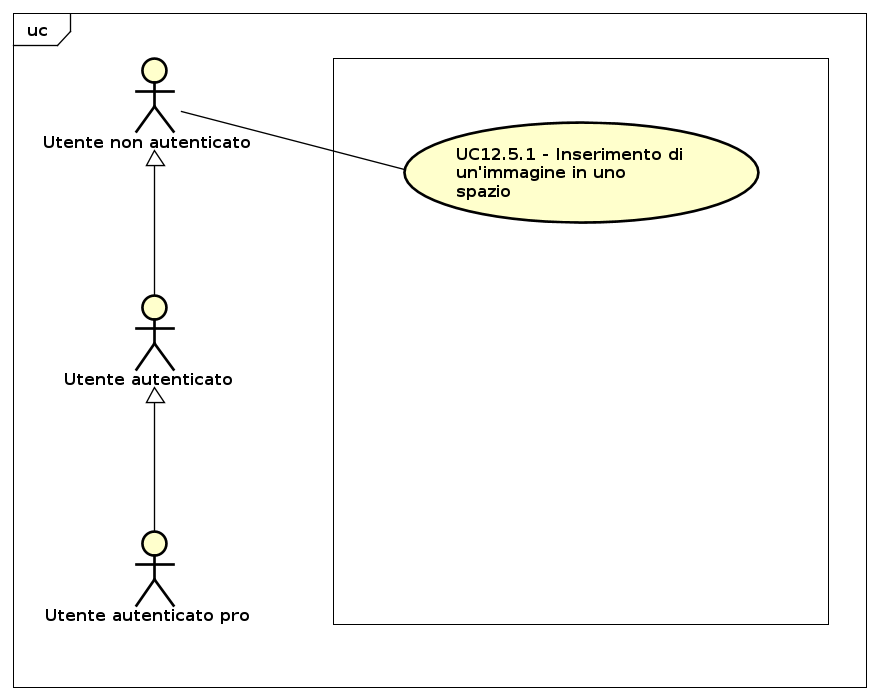
\includegraphics[scale=0.5]{UML/UC12_5.png}
	\caption{UC12.5: Ordinamento di immagini}
\end{figure}
\begin{itemize}
\item \textbf{Attori}: utente autenticato, utente autenticato pro;
\item \textbf{Descrizione}: l'attore può ordinare le immagini secondo il criterio richiesto nella domanda inserendole negli appositi spazi;
\item \textbf{Precondizione}: l'attore visualizza la lista non ordinata delle immagini e la lista vuota in cui andranno inserite;
\item \textbf{Postcondizione}: l'attore ha inserito le immagini nella lista ordinata;
\item \textbf{Scenario principale}: l'attore ordina le immagini secondo il criterio richiesto nella domanda inserendole negli appositi spazi (UC12.5.1).
\end{itemize}

\newpage
\subsubsection{Caso d'uso UC12.5.1: Inserimento di un'immagine in uno spazio}
\label{UC12.5.1}
\begin{figure}[h]
	\centering
	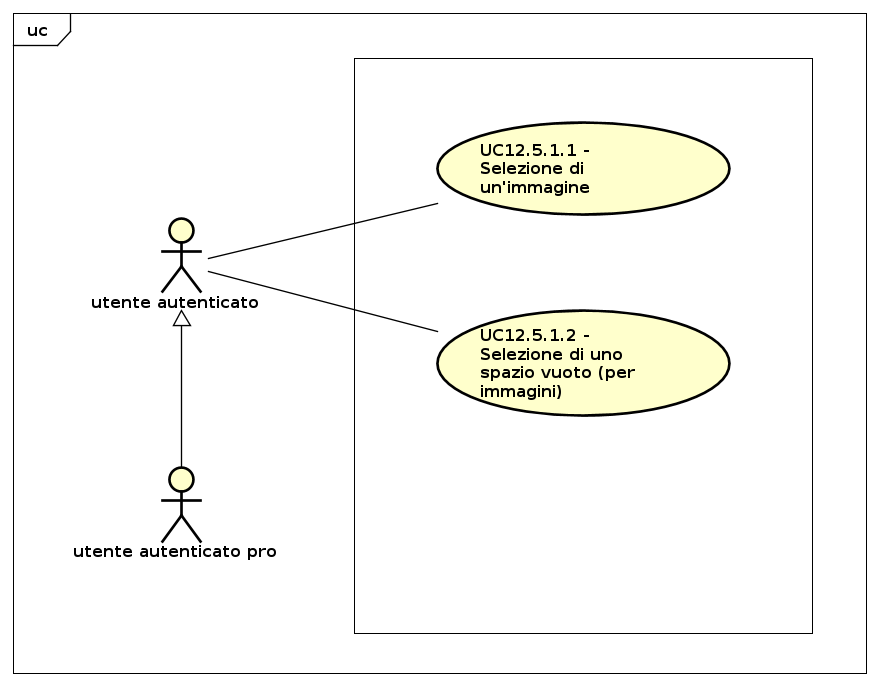
\includegraphics[scale=0.5]{UML/UC12_5_1.png}
	\caption{UC12.5.1: Inserimento di un'immagine in uno spazio}
\end{figure}
\begin{itemize}
\item \textbf{Attori}: utente autenticato, utente autenticato pro;
\item \textbf{Descrizione}: l'attore può selezionare un'immagine per inserirla in uno spazio vuoto o scambiarla con un'altra se lo spazio è già occupato;
\item \textbf{Precondizione}: l'attore visualizza le immagini non ordinate e gli spazi vuoti;
\item \textbf{Postcondizione}: l'attore ha inserito l'immagine nello spazio selezionato;
\item \textbf{Scenario principale}: l'attore seleziona un'immagine (UC12.5.1.1) e la inserisce in uno spazio vuoto o la scambia con un'altra se lo spazio è già occupato (UC12.5.1.2).
\end{itemize}

\subsubsection{Caso d'uso UC12.5.1.1: Selezione di un'immagine}
\begin{itemize}
\item \textbf{Attori}: utente autenticato, utente autenticato pro;
\item \textbf{Descrizione}: l'attore può selezionare un'immagine;
\item \textbf{Precondizione}: l'attore visualizza le immagini non ordinate e gli spazi vuoti;
\item \textbf{Postcondizione}: l'attore ha selezionato un'immagine;
\item \textbf{Scenario principale}: l'attore seleziona un'immagine.
\end{itemize}

\subsubsection{Caso d'uso UC12.5.1.2: Selezione di uno spazio vuoto (per immagini)}
\begin{itemize}
\item \textbf{Attori}: utente autenticato, utente autenticato pro;
\item \textbf{Descrizione}: l'attore può selezionare uno spazio vuoto;
\item \textbf{Precondizione}: l'attore visualizza le immagini non ordinate e gli spazi vuoti;
\item \textbf{Postcondizione}: l'attore ha selezionato uno spazio vuoto;
\item \textbf{Scenario principale}: l'attore seleziona uno spazio vuoto.
\end{itemize}

\subsubsection{Caso d'uso UC12.6: Ordinamento di stringhe}
\label{UC12.6}
\begin{figure}[h]
	\centering
	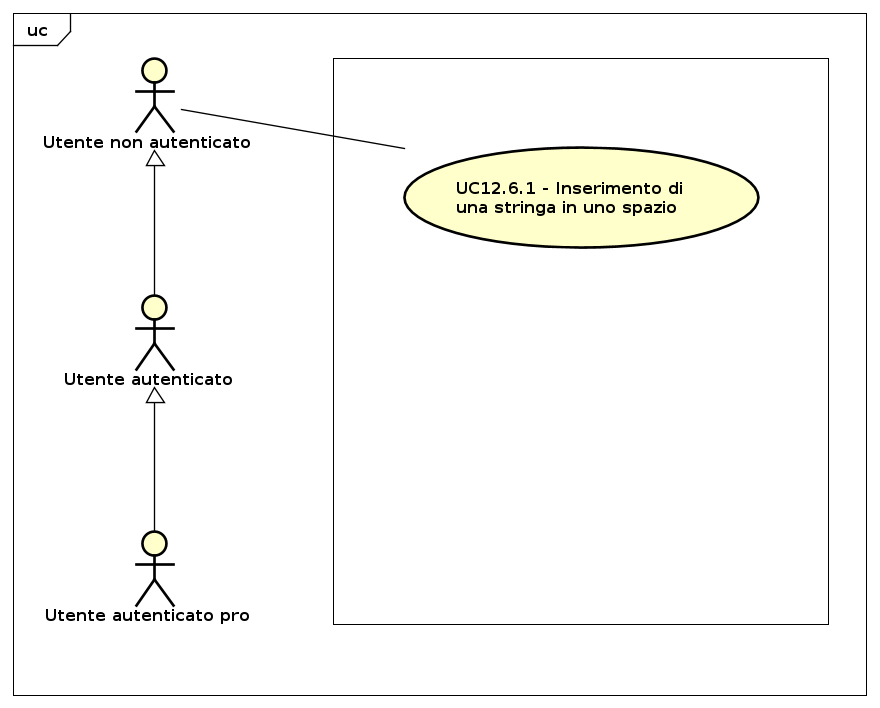
\includegraphics[scale=0.5]{UML/UC12_6.png}
	\caption{UC12.6: Ordinamento di stringhe}
\end{figure}
\begin{itemize}
\item \textbf{Attori}: utente autenticato, utente autenticato pro;
\item \textbf{Descrizione}: l'attore può ordinare le stringhe secondo il criterio richiesto nella domanda inserendole negli appositi spazi;
\item \textbf{Precondizione}: l'attore visualizza la lista non ordinata delle stringhe e la lista vuota in cui andranno inserite;
\item \textbf{Postcondizione}: l'attore ha inserito le stringhe nella lista ordinata;
\item \textbf{Scenario principale}: l'attore ordina le stringhe secondo il criterio richiesto nella domanda inserendole negli appositi spazi (UC12.6.1).
\end{itemize}

\newpage
\subsubsection{Caso d'uso UC12.6.1: Inserimento di una stringa in uno spazio}
\label{UC12.6.1}
\begin{figure}[h]
	\centering
	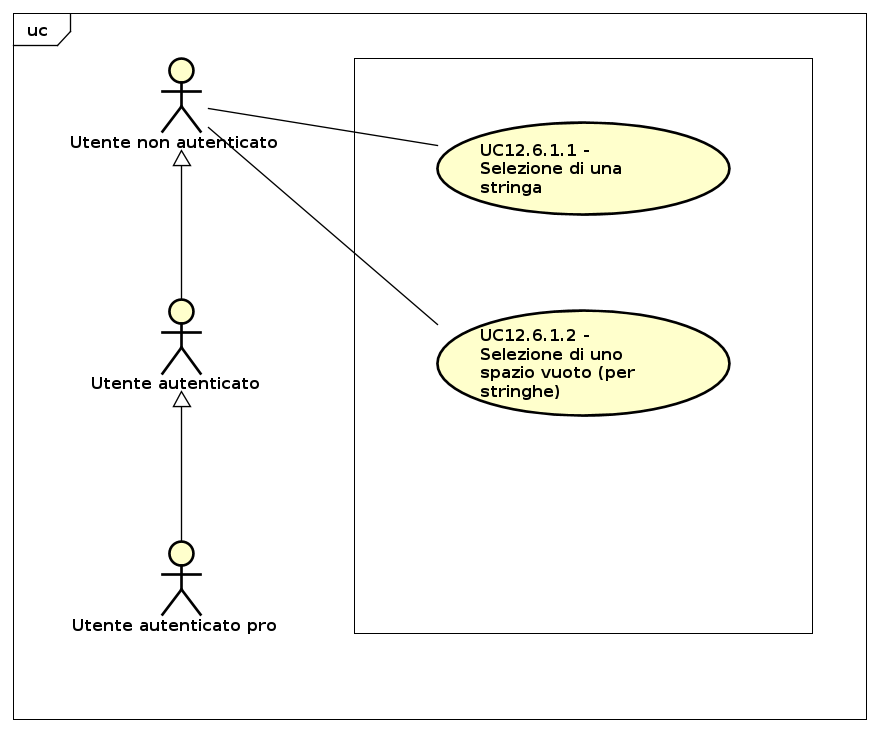
\includegraphics[scale=0.5]{UML/UC12_6_1.png}
	\caption{UC12.6.1: Inserimento di una stringa in uno spazio}
\end{figure}
\begin{itemize}
\item \textbf{Attori}: utente autenticato, utente autenticato pro;
\item \textbf{Descrizione}: l'attore può selezionare una stringa per inserirla in uno spazio vuoto o scambiarla con un'altra se lo spazio è già occupato;
\item \textbf{Precondizione}: l'attore visualizza le stringhe non ordinate e gli spazi vuoti;
\item \textbf{Postcondizione}: l'attore ha inserito la stringa nello spazio selezionato;
\item \textbf{Scenario principale}: l'attore seleziona una stringa (UC12.6.1.1) e la inserisce in uno spazio vuoto o la scambia con un'altra se lo spazio è già occupato (UC12.6.1.2).
\end{itemize}

\subsubsection{Caso d'uso UC12.6.1.1: Selezione di una stringa}
\begin{itemize}
\item \textbf{Attori}: utente autenticato, utente autenticato pro;
\item \textbf{Descrizione}: l'attore può selezionare una stringa;
\item \textbf{Precondizione}: l'attore visualizza le stringhe non ordinate e gli spazi vuoti;
\item \textbf{Postcondizione}: l'attore ha selezionato una stringa;
\item \textbf{Scenario principale}: l'attore seleziona una stringa.
\end{itemize}

\subsubsection{Caso d'uso UC12.6.1.2: Selezione di uno spazio vuoto (per stringhe)}
\begin{itemize}
\item \textbf{Attori}: utente autenticato, utente autenticato pro;
\item \textbf{Descrizione}: l'attore può selezionare uno spazio vuoto;
\item \textbf{Precondizione}: l'attore visualizza le stringhe non ordinate e gli spazi vuoti;
\item \textbf{Postcondizione}: l'attore ha selezionato uno spazio vuoto;
\item \textbf{Scenario principale}: l'attore seleziona uno spazio vuoto.
\end{itemize}

\subsubsection{Caso d'uso UC12.7: Risposta ad una domanda con area cliccabile}
\label{UC12.7}
\begin{figure}[h]
	\centering
	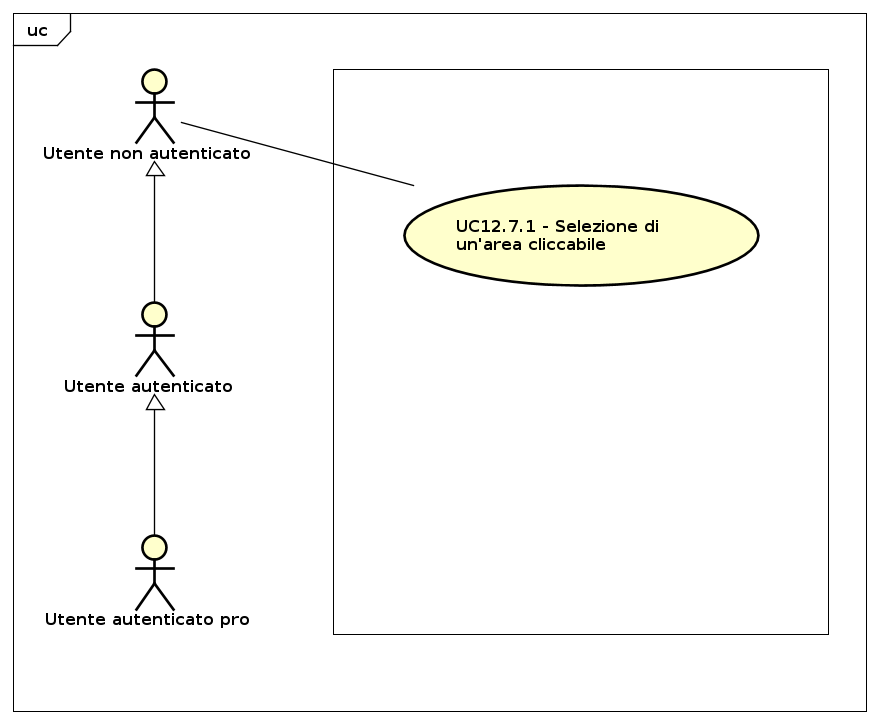
\includegraphics[scale=0.5]{UML/UC12_7.png}
	\caption{UC12.7: Risposta ad una domanda con area cliccabile}
\end{figure}
\begin{itemize}
\item \textbf{Attori}: utente autenticato, utente autenticato pro;
\item \textbf{Descrizione}: l'attore può selezionare una o più aree cliccabili;
\item \textbf{Precondizione}: l'attore visualizza la domanda con area cliccabile;
\item \textbf{Postcondizione}: l'attore ha risposto alla domanda con area cliccabile;
\item \textbf{Scenario principale}: l'attore seleziona una o più aree cliccabili (UC12.7.1).
\end{itemize}

\subsubsection{Caso d'uso UC12.7.1: Selezione di un'area cliccabile}
\begin{itemize}
\item \textbf{Attori}: utente autenticato, utente autenticato pro;
\item \textbf{Descrizione}: l'attore può selezionare un'area cliccabile;
\item \textbf{Precondizione}: l'attore visualizza le aree cliccabili;
\item \textbf{Postcondizione}: l'attore ha selezionato un'area cliccabile;
\item \textbf{Scenario principale}: l'attore seleziona un'area cliccabile.
\end{itemize}

\newpage
\subsection{Caso d'uso UC13: Ricerca utente}
\label{UC13}
\begin{figure}[h]
	\centering
	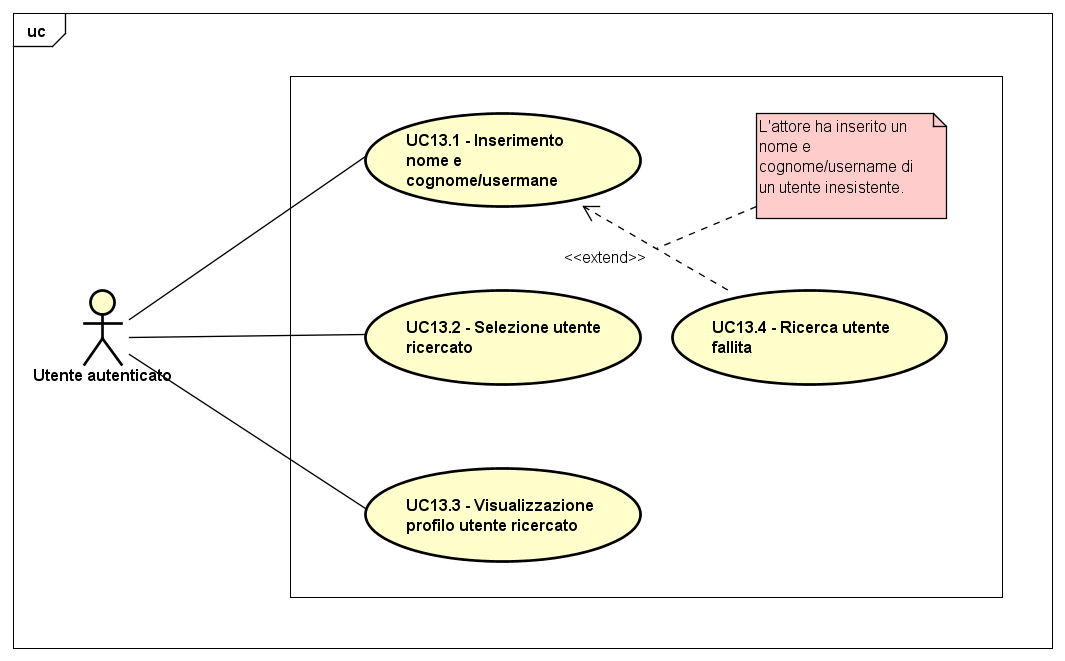
\includegraphics[scale=0.5]{UML/UC13.png}
	\caption{UC13: Ricerca utente}
\end{figure}
\FloatBarrier
\begin{itemize}
	\item \textbf{Attori}: utente autenticato, utente autenticato pro;
	\item \textbf{Descrizione}: l'attore può ricercare un utente registrato al sistema;
	\item \textbf{Precondizione}: l'attore si trova nella pagina iniziale;
	\item \textbf{Postcondizione}: il sistema visualizza il profilo dell'utente ricercato;
	\item \textbf{Scenario principale}:
	\begin{enumerate}
		\item L'attore può inserire nome e cognome/username dell'utente che vuole ricercare (UC13.1);
		\item L'attore può selezionare l'utente ricercato per visualizzarne il profilo (UC13.2).
	\end{enumerate} 
	\item \textbf{Estensioni}: la ricerca dell'utente è fallita (UC13.3);
	\item \textbf{Scenari alternativi}: l'utente ha inserito nella barra di ricerca un nome e cognome/username inesistente all'interno del sistema. 
\end{itemize}

\subsubsection{Caso d'uso UC13.1: Inserimento nome e cognome/usermane}

\begin{itemize}
	\item \textbf{Attori}: utente autenticato, utente autenticato pro;
	\item \textbf{Descrizione}: l'attore può inserire nome e cognome/username di un utente nella barra di ricerca;
	\item \textbf{Precondizione}: l'attore ha selezionato la barra di ricerca utente;
	\item \textbf{Postcondizione}: l'attore ha inserito nome e cognome/username dell'utente che vuole ricercare;
	\item \textbf{Scenario principale}: l'attore inserisce il nome e cognome/username dell'utente che vuole ricercare.
\end{itemize}

\subsubsection{Caso d'uso UC13.2: Selezione utente ricercato}

\begin{itemize}
	\item \textbf{Attori}: utente autenticato, utente autenticato pro;
	\item \textbf{Descrizione}: l'attore può selezionare l'utente ricercato per visualizzarne il profilo;
	\item \textbf{Precondizione}: l'utente ha inserito il nome e congome/username dell'utente ricercato nella barra di ricerca;
	\item \textbf{Postcondizione}: il sistema visualizza il profilo dell'utente selezionato;
	\item \textbf{Scenario principale}: l'attore seleziona l'utente ricercato per visualizzarne il profilo.
\end{itemize}

\subsubsection{Caso d'uso UC13.3: Ricerca utente fallita}

\begin{itemize}
	\item \textbf{Attori}: utente autenticato, utente autenticato pro;
	\item \textbf{Descrizione}: l'attore può visualizzare un messaggio d'errore nel caso si fosse verificato lo scenario alternativo durante la fase di ricerca dell'utente;
	\item \textbf{Precondizione}: l'attore ha inserito nome e cognome/username di un utente inesistente;
	\item \textbf{Postcondizione}: il sistema avvisa l'attore dell'errore verificatosi tramite un opportuno messaggio;
\item\textbf{Scenario principale}: l'attore visualizza un messaggio d'errore.
\end{itemize}

\newpage
\subsection{Caso d'uso UC14: Login con Facebook}
\label{UC14}
\begin{figure}[ht]
	\centering
	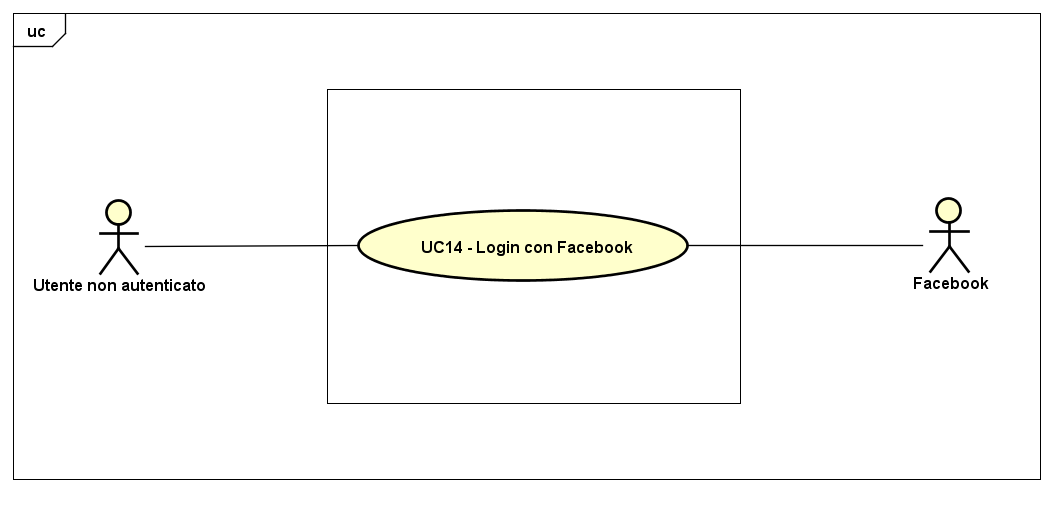
\includegraphics[scale=0.48]{UML/UC14.png}
	\caption{UC14: Login da Facebook}
\end{figure}
\FloatBarrier
\begin{itemize}
	\item \textbf{Attori}: utente non autenticato, Facebook;
	\item \textbf{Descrizione}: l'attore può autenticarsi utilizzando Facebook;
	\item \textbf{Precondizione}: l'attore visualizza la pagina di login e sceglie il login con Facebook;
	\item \textbf{Postcondizione}: l'attore è autenticato;
	\item \textbf{Scenario principale}: l'attore effettua il login tramite Facebook.
\end{itemize}


\newpage
\subsection{Caso d'uso UC15: Login con Twitter}
\label{UC15}
\begin{figure}
	\centering
	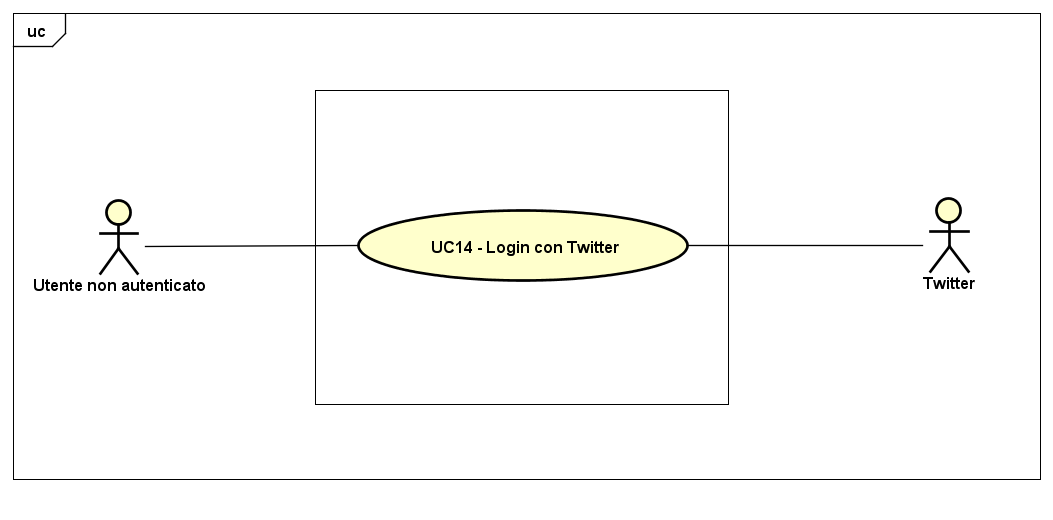
\includegraphics[scale=0.48]{UML/UC15.png}
	\caption{UC15: Login da Twitter}
\end{figure}
\FloatBarrier
\begin{itemize}
	\item \textbf{Attori}: utente non autenticato, Twitter;
	\item \textbf{Scopo e descrizione}: l'attore può autenticarsi utilizzando Twitter;
	\item \textbf{Precondizione}: l'attore visualizza la pagina di login e sceglie il login con Twitter;
	\item \textbf{Postcondizione}: l'attore è autenticato;
	\item \textbf{Scenario principale}: l'attore effettua il login tramite Twitter.
\end{itemize}


\newpage
\subsection{Caso d'uso UC16: Login con Google+}
\label{UC16}
\begin{figure}[ht]
	\centering
	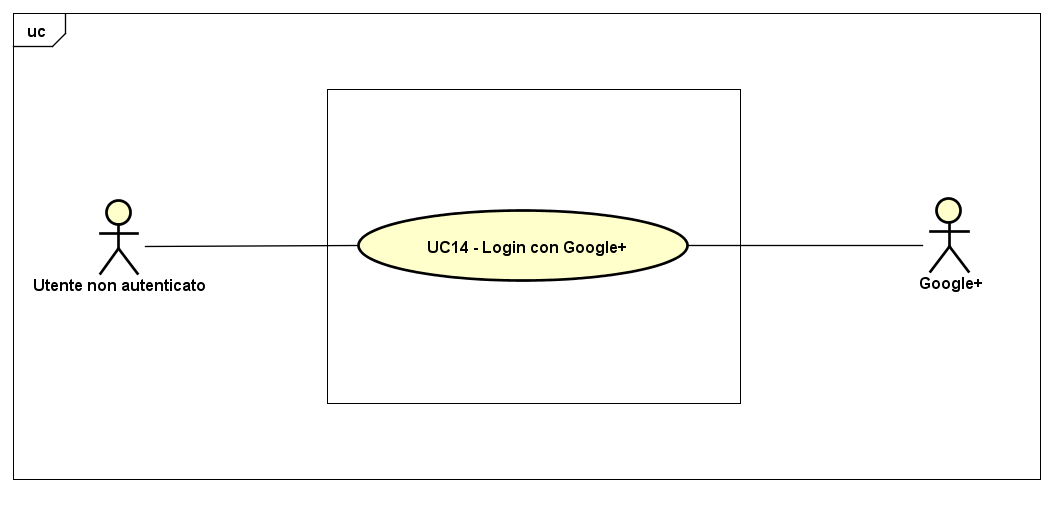
\includegraphics[scale=0.48]{UML/UC16.png}
	\caption{UC16: Login da Google+}
\end{figure}
\FloatBarrier
\begin{itemize}
	\item \textbf{Attori}: utente non autenticato, Google+;
	\item \textbf{Descrizione}: l'attore può autenticarsi utilizzando Google+;
	\item \textbf{Precondizione}: l'attore visualizza la pagina di login e sceglie il login con Google+;
	\item \textbf{Postcondizione}: l'attore è autenticato;
	\item \textbf{Scenario principale}: l'attore effettua il login tramite Google+.
\end{itemize}


\newpage
\subsection{Caso d'uso UC17: Login con LinkedIn}
\label{UC17}
\begin{figure}
	\centering
	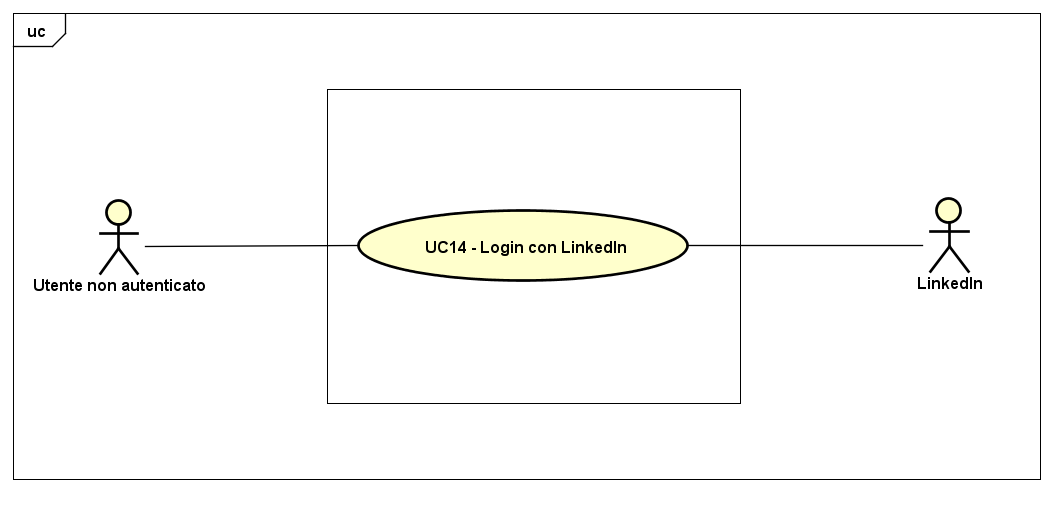
\includegraphics[scale=0.48]{UML/UC17.png}
	\caption{UC17: Login da LinkedIn}
\end{figure}
\FloatBarrier
\begin{itemize}
	\item \textbf{Attori}: utente non autenticato, LinkedIn;
	\item \textbf{Descrizione}: l'attore può autenticarsi utilizzando LinkedIn;
	\item \textbf{Precondizione}: l'attore visualizza la pagina di login e sceglie il login con LinkedIn;
	\item \textbf{Postcondizione}: l'attore è autenticato;
	\item \textbf{Scenario principale}: l'attore effettua il login tramite LinkedIn.
\end{itemize}